\documentclass[nojss]{jss}\usepackage[]{graphicx}\usepackage[]{color}
% maxwidth is the original width if it is less than linewidth
% otherwise use linewidth (to make sure the graphics do not exceed the margin)
\makeatletter
\def\maxwidth{ %
  \ifdim\Gin@nat@width>\linewidth
    \linewidth
  \else
    \Gin@nat@width
  \fi
}
\makeatother

\definecolor{fgcolor}{rgb}{0.345, 0.345, 0.345}
\newcommand{\hlnum}[1]{\textcolor[rgb]{0.686,0.059,0.569}{#1}}%
\newcommand{\hlstr}[1]{\textcolor[rgb]{0.192,0.494,0.8}{#1}}%
\newcommand{\hlcom}[1]{\textcolor[rgb]{0.678,0.584,0.686}{\textit{#1}}}%
\newcommand{\hlopt}[1]{\textcolor[rgb]{0,0,0}{#1}}%
\newcommand{\hlstd}[1]{\textcolor[rgb]{0.345,0.345,0.345}{#1}}%
\newcommand{\hlkwa}[1]{\textcolor[rgb]{0.161,0.373,0.58}{\textbf{#1}}}%
\newcommand{\hlkwb}[1]{\textcolor[rgb]{0.69,0.353,0.396}{#1}}%
\newcommand{\hlkwc}[1]{\textcolor[rgb]{0.333,0.667,0.333}{#1}}%
\newcommand{\hlkwd}[1]{\textcolor[rgb]{0.737,0.353,0.396}{\textbf{#1}}}%
\let\hlipl\hlkwb

\usepackage{framed}
\makeatletter
\newenvironment{kframe}{%
 \def\at@end@of@kframe{}%
 \ifinner\ifhmode%
  \def\at@end@of@kframe{\end{minipage}}%
  \begin{minipage}{\columnwidth}%
 \fi\fi%
 \def\FrameCommand##1{\hskip\@totalleftmargin \hskip-\fboxsep
 \colorbox{shadecolor}{##1}\hskip-\fboxsep
     % There is no \\@totalrightmargin, so:
     \hskip-\linewidth \hskip-\@totalleftmargin \hskip\columnwidth}%
 \MakeFramed {\advance\hsize-\width
   \@totalleftmargin\z@ \linewidth\hsize
   \@setminipage}}%
 {\par\unskip\endMakeFramed%
 \at@end@of@kframe}
\makeatother

\definecolor{shadecolor}{rgb}{.97, .97, .97}
\definecolor{messagecolor}{rgb}{0, 0, 0}
\definecolor{warningcolor}{rgb}{1, 0, 1}
\definecolor{errorcolor}{rgb}{1, 0, 0}
\newenvironment{knitrout}{}{} % an empty environment to be redefined in TeX

\usepackage{alltt}

%% -- LaTeX packages and custom commands ---------------------------------------

%% recommended packages
\usepackage{thumbpdf,lmodern}

%% another package (only for this demo article)
\usepackage{framed}
\usepackage{amsmath}
\usepackage{amssymb}
\usepackage{multirow}
\usepackage{booktabs}
\usepackage{soul} % for highlightinh in review process
\usepackage{xcolor}
\usepackage{color}
\usepackage{footnote}
%\usepackage{ulem}
%% new custom commands
\newcommand{\class}[1]{`\code{#1}'}
\newcommand{\fct}[1]{\code{#1()}}
\newcommand{\green}[1]{\textcolor{green}{#1}}
\newcommand{\magenta}[1]{\textcolor{magenta}{#1}}
\newcommand{\orange}[1]{\textcolor{orange}{#1}}
\newcommand{\cyan}[1]{\textcolor{cyan}{#1}}
\DeclareRobustCommand{\hlb}[1]{{\sethlcolor{cyan}\hl{#1}}}


%% -- Article metainformation (author, title, ...) -----------------------------

%% - \author{} with primary affiliation
%% - \Plainauthor{} without affiliations
%% - Separate authors by \And or \AND (in \author) or by comma (in \Plainauthor).
%% - \AND starts a new line, \And does not.
\author{Alexander Lange\\University of Goettingen
    \And Bernhard Dalheimer\\University of Goettingen
    \AND Helmut Herwartz\\University of Goettingen
	\And Simone Maxand\\University of Helsinki
   }
\Plainauthor{Alexander Lange, Bernhard Dalheimer, Helmut Herwartz, Simone Maxand}
%\Plainauthor{Simone Maxand, Second Author}

%% - \title{} in title case
%% - \Plaintitle{} without LaTeX markup (if any)
%% - \Shorttitle{} with LaTeX markup (if any), used as running title
\title{\pkg{svars}: An \proglang{R} Package for Data-Driven Identification in Multivariate Time Series Analysis}
\Plaintitle{svars: An R Package for Data-Driven Identification in Multivariate Time Series Analysis}
\Shorttitle{\pkg{svars}: An \proglang{R} Package for Data-Driven Identification in Multivariate Time Series Analysis}

%% - \Abstract{} almost as usual
\Abstract{Structural vector autoregressive (SVAR) models are frequently applied to trace the contemporaneous linkages among (macroeconomic) variables back to an interplay of orthogonal structural shocks. Under Gaussianity the structural parameters are unidentified without additional (often external and not data-based) information. In contrast, the often reasonable assumption of heteroskedastic and/or non-Gaussian model disturbances offers the possibility to identify unique structural shocks. We describe the \proglang{R} package \pkg{svars} which implements statistical identification techniques that can be both heteroskedasticity based or independence based. Moreover, it includes a rich variety of analysis tools that are well known in the SVAR literature. Next to a comprehensive review of the theoretical background, we provide a detailed description of the associated \proglang{R} functions. Furthermore, a macroeconomic application serves as a step-by-step guide on how to apply these functions to the identification and interpretation of structural VAR models.
}

%% - \Keywords{} with LaTeX markup, at least one required
%% - \Plainkeywords{} without LaTeX markup (if necessary)
%% - Should be comma-separated and in sentence case.
\Keywords{SVAR models, identification, independent components, non-Gaussian maximum likelihood, changes in volatility, smooth transition covariance, \proglang{R}}
\Plainkeywords{JSS, style guide, comma-separated, not capitalized, R}

%% - \Address{} of at least one author
%% - May contain multiple affiliations for each author
%%   (in extra lines, separated by \emph{and}\\).
%% - May contain multiple authors for the same affiliation
%%   (in the same first line, separated by comma).
\Address{
  Alexander Lange\\
  Chair of Econometrics\\
  Faculty of Economic Science\\
  Universitaet Goettingen\\
  Humboldtallee 3\\
  37073 Goettingen, Germany\\
}
\IfFileExists{upquote.sty}{\usepackage{upquote}}{}
\begin{document}
%\linespread{3.0}\selectfont % Zum ändern des Zeilenabstandes

%% -- Introduction -------------------------------------------------------------

%% - In principle "as usual".
%% - But should typically have some discussion of both _software_ and _methods_.
%% - Use \proglang{}, \pkg{}, and \code{} markup throughout the manuscript.
%% - If such markup is in (sub)section titles, a plain text version has to be
%%   added as well.
%% - All software mentioned should be properly \cite-d.
%% - All abbreviations should be introduced.
%% - Unless the expansions of abbreviations are proper names (like "Journal
%%   of Statistical Software" above) they should be in sentence case (like
%%   "generalized linear models" below).

\section[Introduction]{Introduction} \label{sec:intro}

Particularly in macroeconometrics, structural vector autoregressive (SVAR) models have become a prominent tool to determine the impacts of different (economic) shocks in a system of variables. Within these models, the unobserved structural shocks represent information that is hidden in the reduced form vector autoregressive (VAR) model. Nevertheless, analysts might be interested in the system's reaction to exactly this type of isolated shocks, which is commonly visualized by means of impulse-response functions. For instance, policy makers could be interested in revealing the effects of an unexpected interest rate cut. Estimating the reduced form VAR by means of least squares (LS) or maximum likelihood methods (ML) is straightforward \citep[see, e.g.,][]{IntroductionMultipleTS}, however, identifying the non-unique structural form is a controversial topic in the SVAR literature. %ecause it cannot be recovered directly from the data.

Beginning with the pioneering work of \cite{Sims1980}, two main types of identification strategies have been developed. On the one hand, following \cite{Sims1980} original ideas such strategies refer to economic theory. Theory based methods implement economic restrictions (e.g., short-run restrictions \citep{Sims1980}, long-run restrictions \citep{BlacnchardQuah1989} or specific sign patterns \citep{Uhlig2005}) a-priori. On the other hand,  statistical identification methods which have been developed more recently exploit the informational content of specific data features (heteroskedasticitiy of structural shocks, uniqueness of non-Gaussian independent components).  The \proglang{R} package \pkg{svars}, which we describe in this paper, focuses on these statistical methods to identify the structural shocks.%However, the data might not support the economic restrictions, which leads to an incorrect further analysis.

The \proglang{R} \citep{R} archive network comprises several widely applied packages for multivariate time series models and, in particular, for analyzing VAR models. The \pkg{vars} package \citep{pfaff2008} contains estimation techniques for reduced form VAR models, and functions to determine the lag order and to perform several diagnostic tests. Moreover, the \pkg{vars} package allows for the estimation of a basic structural form by means of theory-based short- and long-run restrictions. Further \proglang{R} packages for multivariate time series analysis and VAR estimation are \pkg{tsDyn} \citep{tsDyn} and \pkg{MTS} \citep{MTS}. To the authors' knowledge, currently only the \pkg{VARsignR} package \citep{VARsignR} contains functions for SVAR identification by means of theory-based sign restrictions.

Given the lack of implementations of statistical identification techniques in \proglang{R}, the package \pkg{svars} has been explicitly developed to fill this gap by providing various recent statistical methods to estimate SVAR models. These methods build upon distinct but not mutually exclusive statistical properties of the data (i.e., covariance changes and the uniqueness of independent non-Gaussian distributed structural shocks). The \pkg{svars} package supports six identification techniques. Three identification methods make use of the assumption of heteroskedastic shocks, i.e., the identification (i)  via changes in volatility \citep{Rigobon2003}, (ii) via smooth transitions of covariances \citep{LUTKEPOHL201743} and (iii) via generalized autoregressive conditional heteroskedasticity (GARCH) \citep{NP2004, BouakezNormadin2010}. Three further identification methods connect to the uniqueness of non-Gaussian independent components, namely the   detection of least dependent innovations based on  (iv) Cram\'er-von Mises (CVM) statistics \citep{HerwartzLDI2018}, (v) the distance covariances  \citep{Matteson2017} and (vi) a parametric  non-Gaussian  ML approach \citep{LMS2017}.

By offering a variety of identification methods, the \pkg{svars} package can be applied in diverse data settings. Additionally, it extends the existing pool of SVAR techniques in \proglang{R} with more recent bootstrap procedures, further statistics and hypothesis tests directly related to inference in SVAR models. In this sense, the \pkg{svars} package is designed as a complete toolbox for the structural analysis of multivariate time series. Based on objects from reduced form estimations, \pkg{svars} is compatible with other packages such as \pkg{vars}, \pkg{tsDyn} and \pkg{MTS}. Moreover, computationally demanding modules are fully implemented in \proglang{C++} and linked to \proglang{R} using the \pkg{Rcpp} \citep{Rcpp} and \pkg{RcppArmadillo }\citep{arma2014} libraries. The package is available on CRAN at \href{https://cran.r-project.org/package=svars}{https://cran.r-project.org/package=svars}. \\

The article is organized as follows: Section \ref{sec:models} outlines the SVAR model and the alternative identification methods. In Section \ref{sec:tools}, we describe bootstrap methods and further diagnostic tools for SVAR analysis. Section \ref{sec:pkg_structure} details the package design, and Section \ref{sec:Example} provides an illustrative application of two identification schemes to a real world dataset. Lastly, a summary and an outlook on future extensions of the \pkg{svars} package complete this article.

%% -- Manuscript ---------------------------------------------------------------

%% - In principle "as usual" again.
%% - When using equations (e.g., {equation}, {eqnarray}, {align}, etc.
%%   avoid empty lines before and after the equation (which would signal a new
%%   paragraph.
%% - When describing longer chunks of code that are _not_ meant for execution
%%   (e.g., a function synopsis or list of arguments), the environment {Code}
%%   is recommended. Alternatively, a plain {verbatim} can also be used.
%%   (For executed code see the next section.)

\section{Structural vector autoregressive models} \label{sec:models}

{Consider a $K$-dimensional VAR model of order $p$
\begin{align}
y_t &= \mu + A_1y_{t-1} + ... + A_py_{t-p} + u_t,\label{eq:VAR}\\
&= \mu + A_1y_{t-1} + ... + A_py_{t-p} + B\varepsilon_t, \qquad t = 1,..., T,\label{eq:VAR2}
%\Leftrightarrow B^{-1}y_t &= B^{-1}\mu + B^{-1}A_1y_{t-1} + ... + B^{-1}A_py_{t-p} + \varepsilon_t, \qquad t = 1,..., T,\label{eq:VAR2}
\end{align}
where $y_t = [y_{1t}, ..., y_{Kt}]^\top$ is a vector of observable variables, $A_i, i=1,\ldots,p,$ are $(K \times K)$ coefficient matrices, and intercept parameters are collected in $\mu$. We focus on the case of time invariant deterministic terms for notational clarity. Model augmentation with time-varying deterministic terms (e.g., breaks, linear trends), however, is straightforward. Furthermore, the VAR model is stationary (invertible) by assumption. The vector $u_t$ consists of reduced-form residuals, which are serially uncorrelated with $\mathbb{E}(u_t) = 0$ and $\mbox{Cov}(u_{t}) = \Sigma_u$.
%\textcolor{orange}{The SVAR model is obtained by premultiplying the matrix $B^{-1}$ to the model equation as displayed in Equation \ref{eq:VAR2}.STIMMT DOCH GAR NICHT? SO EIN SVAR HABE ICH SELTEN GESEHEN?!? DIESEN SATZ BRAUCHEN WIR NULL; OR???}
The nonsingular matrix $B$ captures the instantaneous effects of the structural shocks $\varepsilon_t = B^{-1}u_t$ on the variables of the system.\\}
In the following, we briefly discuss the identification problem in SVAR analysis. Subsequently, we present six alternative statistical approaches to uniquely determine the structural shocks. Finally, we provide a short guidance on how to choose between these alternative identification approaches.

\subsection{The identification problem}

Cross-equation relations between the reduced-form residuals in Equation \ref{eq:VAR} are characterized by the covariance matrix
\begin{equation}\label{eq:CovDec}
\mbox{Cov}(u_t) = \Sigma_u = B\Sigma_\varepsilon B^\top,
\end{equation}
where the covariance of the structural shocks $\mbox{Cov}(\varepsilon_{t}) = \Sigma_\varepsilon$ is a diagonal matrix. Thus, structural shocks are uncorrelated, which enables a meaningful impulse-response analysis \citep{IntroductionMultipleTS}. Without any further model specification, Equation \ref{eq:CovDec} holds for every matrix $B$ which decomposes the covariance matrix $\Sigma_u$. Hence, additional restrictions are necessary to identify a (unique) matrix $B$.\footnote{The identification problem is described in more detail, for instance, in Chapter 1 of \cite{IntroductionMultipleTS}. \cite{LK17} resume a variety of traditional and more recent methods to identify the structural shocks.} In this paper, we focus on  identification techniques which use the underlying data structure to determine the structural matrix. %To identify the structural matrix $B$ and the corresponding structural errors $\varepsilon_t$, one has to rely on economic based- or statistical methods.
After estimating the model in Equation \ref{eq:VAR} by means of LS or ML methods, the resulting reduced form residual estimates $\hat{u}_t$ and the corresponding covariance estimate $\widehat{\Sigma}_u$ provide the starting point for the subsequent identification techniques. The following two Sections introduce the statistical identification methods which constitute the core functions of the \pkg{svars} package. \\


\subsection{Identification by means of heteroskedastic innovations}

Time series are often characterized by time-varying covariance structures. Therefore, it is tempting to unravel the structural relationships by means of such changes in the second order moments \citep[see, e.g.,][]{SF2001, Rigobon2003}. The \pkg{svars} package includes three alternative heteroskedasticity based SVAR identification schemes. The first approach is built upon unconditional shifts in the covariance \citep{Rigobon2003}, while the second procedure allows for a smooth transition between the covariance regimes \citep{LUTKEPOHL201743}. The third scheme implements the identification of the structural shocks via conditional heteroskedasticity \citep{NP2004}.

\subsubsection{Changes in volatility (CV)}\label{cv}

\cite{Rigobon2003} uses the presence of shifts in the time series' variance at known time points for the identification of structural shocks. He considers a model of exogenous covariance changes. More precisely, the changes of the covariance matrix occur at prespecified break dates implying
$$
\mathbb{E}(u_tu_t^\top) = \Sigma_t = \Sigma_u(m) \; \mbox{ for } \; m = 1,...,M,\, t=1,\ldots,T.
$$
Here, the index $m=1,\ldots,M$ indicates the respective variance regime. In the most simple framework of two volatility states (i.e., $M = 2$) with a structural break at time point $T_{sb}\in\{1,\ldots,T\}$, the reduced form covariance matrix is
$$
\mathbb{E}(u_tu_t^\top) =
\begin{cases}
\Sigma_1 \mbox{ for } t = 1,...,T_{sb}-1\\
\Sigma_2 \mbox{ for } t = T_{sb},...,T,
\end{cases}
$$
%Consequently, the first regime is characterized by the covariance matrix $\Sigma_1$ and the second regime by $\Sigma_2$,
where $\Sigma_1 \neq \Sigma_2$. The two covariance matrices can be decomposed as $\Sigma_1 = BB^\top$ and $\Sigma_2 = B\Lambda B^\top$, where %$B$ is a $(K\times K)$ matrix and
$\Lambda$ is a diagonal matrix with diagonal elements $\lambda_{ii} > 0, i = 1,...,K$. The matrix $\Lambda$ formalizes the change of the variance of structural shocks $\varepsilon_t$ in the second regime. In other words, the structural shocks have unit variance in the first regime, and variances $\lambda_{ii}, i=1,\ldots,K,$ in the second regime. The structural shocks are uniquely identified if all diagonal elements in $\Lambda$ are distinct. Under the assumption of Gaussian residuals $u_t$, the log-likelihood function for the estimation of $B$ and $\Lambda$ is
\begin{align}
\log \mathcal{L} &= T\frac{K}{2}\log 2\pi - \frac{T_{sb} - 1}{2}\left[\log \det(BB^\top) + \text{tr}\left(\widehat{\Sigma}_1(BB^\top)^{-1}\right)\right] \nonumber \\
                 &\quad - \frac{T - T_{sb} + 1}{2}\left[\log \det(B \Lambda B^\top) + \text{tr}\left(\widehat{\Sigma}_2(B \Lambda B^\top)^{-1}\right)\right],\label{lik_cv}
\end{align}
where $\widehat{\Sigma}_1$ and $\widehat{\Sigma}_2$ are retrieved from estimated residuals $\widehat{u}_t$, respectively, as
$$
\widehat{\Sigma}_1 = \frac{1}{T_{sb} - 1} \sum _{t = 1}^{T_{sb} -1}\widehat{u}_t\widehat{u}_t^\top \qquad \text{and} \qquad \widehat{\Sigma}_2 = \frac{1}{T - T_{sb} + 1} \sum _{t = T_{sb}}^{T}\widehat{u}_t\widehat{u}_t^\top.
$$
 For the numerical log-likelihood optimization of (\ref{lik_cv}), the initial matrix $B$ is the lower triangular decomposition of $T^{-1} \sum^T_{t=1}\widehat{u}_t\widehat{u}_t^\top$, and the initial matrix $\Lambda$ is set to the identity matrix. \cite{LanneLuetkepohl2008} introduce an iterative procedure to improve the estimation precision of this routine. The matrices $\widetilde{B}$ and $\widetilde{\Lambda}$, which are obtained from maximizing the log-likelihood function, are used for iterative generalized least squares (GLS) estimation of the  deterministic and autoregressive parameters
\begin{align*}
\widehat{\beta} &= \mbox{vec}[\widehat{\mu}, \widehat{A}_1, ..., \widehat{A}_p] \\
                 &= \left[\sum^{T_{sb}-1}_{t=1}\left(Z_t Z_t^\top \otimes (\widetilde{B}\widetilde{B}^\top)^{-1}\right) + \sum^{T}_{t=T_{sb}}\left(Z_t Z_t^\top \otimes (\widetilde{B}\widetilde{\Lambda}\widetilde{B}^\top)^{-1}\right) \right]^{-1} \\
                 &\quad \times \left[\sum^{T_{sb}-1}_{t=1}\left(Z_t \otimes (\widetilde{B}\widetilde{B}^\top)^{-1}\right)y_t + \sum^{T}_{t=T_{sb}}\left(Z_t \otimes (\widetilde{B}\widetilde{\Lambda}\widetilde{B}^\top)^{-1}\right)y_t \right],
\end{align*}
where $Z_t^\top = [1, y_{t-1}^\top,...,y_{t-p}^\top]$. Then, the GLS estimator $\widehat{\beta}$ is used to update the covariance estimates by means of $\widehat{u}_t = y_t - (Z_t^\top \otimes I_K)\widehat{\beta}$. This algorithm iterates until the log-likelihood converges. Furthermore, standard errors for the structural parameters can be obtained from the square root of the inverted information matrix \citep{Hamilton1994}.\\
Identification through changes in volatility is conditional on the determination of the variance regimes. If available, the analyst might use external information for the selection of suitable break points ($T_{sb}$). {Typically these are extraordinary events in history which can be associated with a change in data variation \cite[see, e.g.,][]{RS2004}}. Alternatively, the model might be evaluated conditional on a range of alternative break point candidates from which the analyst selects the model with the highest log-likelihood as described in \cite{LS2018}.

\subsubsection{Smooth transition (co)variances (ST)}\label{sec:smoothtransition}
The implementation of identification via smooth transition covariances follows the descriptions in \cite{LUTKEPOHL201743} and generalizes the identification via changes in volatility. The covariance matrix of the error terms $u_t$ consists of several volatility states, and the transition from one state to another is formalized by means of a non-linear function. For two volatility regimes with distinct covariance matrices $\Sigma_1$ and $\Sigma_2$, the covariance structure at time $t$ is
\begin{equation}\label{smoothCov}
\mathbb{E}(u_tu_t^\top) = \Omega_t = \left(1 - G(s_t)\right)\Sigma_1 + G(s_t)\Sigma_2,\quad t=1,\ldots,T.
\end{equation}
In (\ref{smoothCov}), $G(\cdot)$ is the transition function determined by the transition variable $s_t$. While the transition variable is usually deterministic (e.g., $s_t = t$), the model also allows for stochastic transition variables, for instance, lagged dependent variables \citep[see][for more details]{LUTKEPOHL201743}. The most frequently employed transition function is the logistic function proposed by \cite{Maddala1977}, which is of the form
\begin{equation}\label{transition}
G(\gamma, c, s_t) = \left[1 + \exp(- \exp(\gamma)(s_t - c))\right]^{-1}.
\end{equation}
 The coefficient $\gamma$ determines the slope of the function and $c$ is the time point of transition. Based on the covariance structure  in Equation \ref{smoothCov} and Equation \ref{transition}, and the assumption of normally distributed residuals $u_t$, the log-likelihood function reads as
\begin{equation}\label{stlogl}
\log \mathcal{L} = T\frac{K}{2}\log 2\pi - \frac{1}{2}\sum^T_{t=1}\log \det(\Omega_t) - \frac{1}{2}\sum^T_{t=1}u_t^\top\Omega_t^{-1}u_t.
\end{equation}
Grid optimization enables the determination of the transition parameters $\gamma$ and $c$. \cite{LUTKEPOHL201743} suggest an iterative procedure for every pair of parameters ($\gamma$, $c$). The first step is the maximization of the log-likelihood in (\ref{stlogl}) with respect to the structural parameters $B$ and $\Lambda$. In the second step, the estimated matrices $\widetilde{B}$ and $\widetilde{\Lambda}$ are used to re-estimate the reduced form VAR parameters by means of GLS estimation
$$
\widehat{\beta} = \left((Z_t^\top \otimes I_K)W_T(Z_t \otimes I_K)\right)^{-1}(Z_t^\top \otimes I_K)W_Ty,
$$
where $W_T$ is a blockdiagonal $(KT \times KT)$ weighting matrix
$$
W_T =
\begin{bmatrix}
\Omega^{-1}_1 & \cdots & 0 \\
\vdots & \ddots & \vdots \\
0 & \cdots & \Omega^{-1}_T
\end{bmatrix}.
$$
The GLS step obtains $\widehat{\beta}$ to update the covariance estimates by means of $\widehat{u}_t = y_t - (Z_t^\top \otimes I_K)\widehat{\beta}$. The two steps are performed until  the log-likelihood converges. The iterative procedure is evaluated at every parameter pair ($\gamma$, $c$) within a prespecified range. The parameter pair which maximizes the log-likelihood in Equation \ref{stlogl} is considered to provide the best estimate for the true transition. For a more detailed discussion of the parameter choice see \cite{LUTKEPOHL201743}.

\subsubsection{Conditional heteroskedasticity (GARCH)}

As proposed by \cite{NP2004}, \cite{LS2007} and \cite{BouakezNormadin2010} structural shocks are unique if their conditional variances {are of the GARCH type}. For the formal exposition let $\mathcal{F}_t$ denote a filtration that summarizes systemic information which is available until time $t$. Accordingly, the time-varying covariance {can be represented as}
\begin{equation}
\mathbb{E}(u_tu_t^\top|\mathcal{F}_{t-1}) = \Sigma_{t|t-1} = B\Lambda_{t|t-1}B^\top,
\end{equation}
where
\begin{equation}
\Lambda_{t|t-1} = \text{diag}(\sigma^2_{1,t|t-1}, ..., \sigma^2_{K,t|t-1})
\end{equation}
is a $(K \times K)$ matrix with GARCH implied variances on the main diagonal. In the context of SVAR identification typically low order GARCH(1,1) specifications are assumed, such that the individual variances exhibit a dynamic structure as
\begin{equation}\label{equation:GARCH_param}
\sigma^2_{k,t|t-1} = (1 - \gamma_k - g_k) + \gamma_k\varepsilon^2_{k,t-1} + g_k\sigma^2_{k,t-1|t-2}, \qquad k = 1,..,K.
\end{equation}
Higher-order GARCH structures are rarely employed in practice, even though this can be done in principle. Under suitable distributional and parametric restrictions, $\gamma_k > 0$, $g_k \geq 0$ and $\gamma_k + g_k < 1$, the marginal GARCH processes $\varepsilon_{k,t}$ are covariance stationary \citep{MY2013}. \cite{SF2001} have shown that the structural parameters in $B$ are uniquely identified, if there are at least $K-1$ GARCH-type variances present in $\Lambda_{t|t-1}$ . The parameters $\gamma_k$ and $g_k$ can be estimated by means of standard univariate ML approaches. The multivariate Gaussian log-likelihood to obtain the structural parameters in $B$ is
\begin{equation}\label{eq:MGARCH}
\log \mathcal{L} = T\frac{K}{2}\log 2\pi -\frac{1}{2}\sum^T_{t=1}\log\det(\Sigma_{t|t-1}) -\frac{1}{2}\sum^T_{t=1}u^\top_t\Sigma_{t|t-1}u_t.
\end{equation}
For the practical implementation of identification through patterns of conditional heteroskedasticity, we follow the approach suggested by \cite{RePEc:eee:dyncon:v:73:y:2016:i:c:p:241-258}, and estimate the parameters in  (\ref{equation:GARCH_param}) and (\ref{eq:MGARCH}) iteratively until the log-likelihood  in (\ref{eq:MGARCH}) converges.

\subsection{Identification through independent components}

As implied by a result of \cite{Comon1994}, independence of the components of $\varepsilon_t$ could serve to  identify the matrix $B$ if at most one component $\varepsilon_{it}$ exhibits a Gaussian distribution. Furthermore, partial identification of the non-Gaussian components is possible if the system contains multiple Gaussian components \citep[cf.][]{MAXAND2018}. The \pkg{svars} package implements three distinct approaches for identification by means of independent components. Referring to principles of Hodges-Lehman estimation \citep[HL estimation, ][]{HodgesLehman2006}, the first two identification strategies allow for the detection of least dependent structural shocks by the minimization of nonparametric dependence criteria. More specifically, the first technique reveals the structural shocks by minimizing the CVM distance of \cite{Genest2007}. Following a suggestion of \cite{Matteson2017}, the distance covariance statistic of \cite{Szek07} is employed as a nonparametric independence diagnostic for the second estimator. The third identification scheme is a fully parametric ML approach for detecting independent Student-$t$ distributed shocks \citep{LMS2017}.

\subsubsection{Least dependent innovations build on Cram\'er-von Mises statistics (CVM)}

Under Gaussianity, the decomposition factor $B$ of the covariance matrix $\Sigma_u$ is not unique as Gaussian random vectors do not change their joint distribution under rotation. In contrast, assuming not more than one Gaussian distributed component $\varepsilon_{it}$ in $\varepsilon_{t}$, the structural matrix $B$ can be uniquely determined. Introducing the nonparametric identification scheme, let $D$ denote a lower triangular Choleski factor of the covariance matrix of the reduced-form errors, $\Sigma_u = DD^\top$, which links the structural and reduced form errors by $\varepsilon_t = D^{-1}u_t$. Further candidate structural shocks can be generated as
\begin{equation}
\tilde{\varepsilon}_t = Q\varepsilon_t = QD^{-1}u_t,\label{eq:rot_eps}
\end{equation}
where $Q$ is a rotation matrix such that $Q\ne I_K,\,QQ^\top=I_K$. The rotation matrix could be parameterized as the product of $K(K-1)/2$ distinct forms of orthogonal Givens rotation matrices. In the case of $K = 3$, for instance, $Q(\theta)$ is defined as
$$
Q(\theta) =
\begin{bmatrix}
1 & 0 & 0 \\
0 & \cos(\theta_1) & -\sin(\theta_1) \\
0 & \sin(\theta_1) & \cos(\theta_1)
\end{bmatrix}
\times
\begin{bmatrix}
\cos(\theta_2) & 0 & -\sin(\theta_2) \\
0 & 1 & 0 \\
\sin(\theta_2) & 0 & \cos(\theta_2)
\end{bmatrix}
\times
\begin{bmatrix}
\cos(\theta_3) & -\sin(\theta_3) & 0 \\
\sin(\theta_3) & \cos(\theta_3) & 0 \\
0 & 0 & 1
\end{bmatrix},
$$
with  rotation angles $0 \leq \theta_i \leq \pi, \: i = 1,2,3$. By definition, the random vector $\tilde{\varepsilon}_t$ in Equation \ref{eq:rot_eps}  is a rotation of $\varepsilon_t$. The set of possible structural matrices $B(\theta)=D\,Q(\theta)$ is defined in terms of the Choleski factor $D$ and the vector of rotation angles $\theta$ of the Givens matrices $Q(\theta)$.\\
To avoid any restrictive assumption on the distribution of $\varepsilon_t$, nonparametric independence tests are applied to measure the degree of dependence. For instance, the copula-based CVM distance of \cite{Genest2007} has been successfully applied in the  SVAR literature \citep{HerwartPloedt2016II, HerwartzLDI2018} to assess mutual dependence. The CVM distance is
\begin{equation}\label{eq:CVM}
\mathcal{B}_\theta = \int_{(0,1)^K}\left[\sqrt{T}\left(C(\tilde{\varepsilon}) - \prod^K_{i = 1}U(\tilde{\varepsilon}_i)\right)\right]^2d\tilde{\varepsilon},
\end{equation}
where $C$ is the empirical copula and $U$ is the distribution function of a uniformly distributed variable on $\{1/T,\ldots,T/T\}$. The CVM algorithm provides a matrix estimate $\widehat{B}$ such that the rotated structural shocks $\tilde{\varepsilon}_t$ minimize the CVM dependence criterion. Hence, the obtained structural shocks are least dependent according to the statistic in (\ref{eq:CVM}) and the corresponding structural matrix $\widehat{B}$ is the HL estimator. Standard errors for $\widehat{B}$ are obtained by means of  bootstrap procedures as presented in Section \ref{sec:bootstrap}.

\subsubsection{Least dependent innovations build on distance covariance (DC)}

There is a variety of nonparametric criteria available to measure the degree of dependence between random variables, one of which, namely the CVM distance, has been described before. The ICA algorithm by \cite{Matteson2017} provides a matrix estimate $\widehat{B}$ such that the respective structural shocks $\tilde{\varepsilon}_t=\widehat{B}^{-1}\widehat{u}_t$ minimize the distance covariance of \cite{Szek07}, which we denote as $\mathcal{U}_T(\tilde{\varepsilon}_t)$, i.e., the elements in $\tilde{\varepsilon}_t$ are least dependent according to $\mathcal{U}_T(.)$. Similar to the procedure building on the CVM statistic, the set of possible structural matrices $B(\theta)$ is defined in terms of the Choleski factor $D$ and the vector of rotation angles $\theta$ of $Q(\theta)$. The rotation angles  $\tilde{\theta}=\text{argmin}_{\theta}\, \mathcal{U}_T(\tilde{\varepsilon}_t(\theta))$ determine the estimated structural matrix $\widehat{B}=B(\tilde{\theta})$.\footnote{For details on the exact minimization procedure and the empirical definition of the dependence measure we refer to \cite{Matteson2017}.} In the \pkg{svars} package, we take advantage of the function \code{steadyICA} from the \proglang{R} package \pkg{steadyICA} \citep{steadyICA} to estimate $\widehat{B}$. The minimum is determined by means of a gradient algorithm.


\subsubsection{Non-Gaussian maximum likelihood (NGML)}

The identification technique described by \cite{LMS2017} is also based on the assumption of non-Gaussian structural error terms. They propose ML estimation to determine the set of independent structural innovations, which are assumed to exhibit a Student $t$-distribution. Moreover, \cite{LMS2017} suggest a three-step estimation method for computationally demanding situations. The first step consists of LS estimation of the VAR parameters $\beta = \mbox{vec}[\mu, A_1, ..., A_p]$ and of the reduced form residuals {$u_{t}(\widehat{\beta}) = y_t - \widehat{\mu} - \widehat{A}_{1}y_{t-1},...,-\widehat{A}_{p}y_{t-p}$}. In the second step the log-likelihood function is maximized conditional on the  first step estimates $\widehat{\beta}$. The log-likelihood function is
\begin{equation}\label{lik_ngml}
\log \mathcal{L}(\delta) = \log \mathcal{L}(\widehat{\beta}, \delta) = T^{-1}\sum^T_{t =1} l_t(\widehat{\beta}, \delta),
\end{equation}
where
$$
l_t(\widehat{\beta}, \delta) = \sum^K_{i = 1}\log f_i(\sigma^{-1}_i\prime_iB(b)^{-1}u_t(\widehat{\beta}); df_i) - \log \det(B(b)) - \sum^K_{i = 1}\log\sigma_i,$$
and $\prime_i$ is the $i$-th unit vector. The parameter vector of the log-likelihood function is composed of $\widehat{\beta}$ and  $ \delta = (b, \sigma, df)$. Regarding the latter, $b$ is a $K(K-1) \times 1$ vector which contains the off-diagonal elements of the covariance decomposition matrix $B$. The parameters $\sigma_i$ and $df_i$ are the scale and the degrees of freedom parameters of the density function $f_i$ of a Student $t$-distribution, respectively. In the third step, the parameter vector $\delta$ is replaced by the estimate $\tilde{\delta}$ and the log-likelihood
$$
\log \mathcal{L}(\beta) = \log \mathcal{L}(\beta, \widetilde{\delta}) = T^{-1}\sum^T_{t =1} l_t(\beta, \widetilde{\delta})
$$
is maximized.

\subsection{Choice of an adequate identification technique}

In the face of a variety of statistical approaches available to model latent structural relationships, method selection becomes an important step of statistical identification. To facilitate this selection step Table~\ref{tab:ModelChoice} provides an overview of the assumptions on the error terms $\varepsilon_t$ within the alternative identification models. Estimating the structural parameters by means of heteroskedasticity based approaches necessitates the corresponding type of covariance structure. Contrarily, identification through independent components is only possible in  non-Gaussian distributional frameworks. Note that we distinguish between nonparametric models (i.e., CVM and DC) where no further specification of the distribution of the innovations is required and fully parametric ML approaches.

\begin{savenotes}
\begin{table}[!h]
\resizebox{\textwidth}{!}{%
\begin{tabular}{l|cccccc}
\hline
\hline
\multirow{4}{*}{Model} & \multicolumn{6}{c}{Assumptions on} \\
 & \multicolumn{3}{c|}{the variance of $\varepsilon_t$} & \multicolumn{3}{c}{the distribution of $\varepsilon_t$} \\
 & Homoskedasticity & \multicolumn{2}{c|}{Heteroskedasticity} & Gaussian & \multicolumn{2}{c}{Non-Gaussian} \\
 &  & Unconditional & \multicolumn{1}{c|}{Conditional} &  & Arbitrary & $t$-distribution \\ \hline
\multicolumn{7}{l}{Heteroskedasticity}\\
\hspace{1em}CV &  & $\checkmark$ & \multicolumn{1}{c|}{} & $\checkmark$ &  &  \\
\hspace{1em}ST\footnote{Depending on the choice of the transition variable, the ST model can capture unconditional as well as conditional heteroskedasticity \citep{LUTKEPOHL201743}.} &  & $\checkmark$ & \multicolumn{1}{c|}{$\checkmark$} & $\checkmark$ &  &  \\
\hspace{1em}GARCH &  &  & \multicolumn{1}{c|}{$\checkmark$} & $\checkmark$ &  &  \\
\multicolumn{7}{l}{Independence}\\
\hspace{1em}CVM & $\checkmark$ &  & \multicolumn{1}{c|}{} &  & $\checkmark$ &  \\
\hspace{1em}DC & $\checkmark$ &  & \multicolumn{1}{c|}{} &  & $\checkmark$ &  \\
\hspace{1em}NGML & $\checkmark$ &  & \multicolumn{1}{c|}{} &  &  & $\checkmark$ \\
\hline
\end{tabular}%
}
\caption{\label{tab:ModelChoice} Overview of identification models and respective underlying assumptions on the error term $\varepsilon_t$.}
\end{table}
\end{savenotes}

A more detailed discussion on method selection in the context of identification via heteroskedasticity can be found in \cite{LUTKEPOHL20172} and \cite{LS2018}. Moreover, \cite{HLM2019} compare heteroskedasticity and independence based models in a large scale simulation study. They show that identification by means of covariance changes provides precise estimation results if the log-likelihood is correctly specified, whereas under (co)variance misspecification such identification schemes lack efficiency or might suffer from estimation bias. In contrast, simulation based evidence suggests that identification via independent components is more robust with respect to alternative distributional frameworks and heteroskedasticity as long as the innovations are non-Gaussian.

\section{SVAR tests, tools and bootstrap methods}\label{sec:tools}

As a basis for the six identification techniques, the statistical analysis of SVAR models requires a diagnostic analysis of the underlying data structure. The presented package comprises two types of data-driven procedures where the first group assumes heteroskedasticity and the second one non-Gaussianity of the error terms. To decide on Gaussianity of the data a number of normality tests are available in respective \proglang{R} packages \citep[see e.g., \pkg{normtest} and \pkg{ICtest},][]{normtest, ICtest}. Furthermore, the \pkg{svars} package contains several useful tests for SVAR analysis which have not yet been implemented in \proglang{R}. Next we describe the diagnostics and discuss several tools which support the economic interpretations of SVAR estimation results.

\subsection{Tests for structural breaks}
As described in Section \ref{sec:models}, identification based on changes in volatility presumes at least one break point to occur in the covariance structure. To detect different types of breaks in the data, several tests that have been implemented in the \pkg{strucchange} package \citep{zeileis2002} are accessible for VAR analysis via the method \code{stability()} of the \pkg{vars} package. In the following, we consider two additional types of multivariate Chow tests, the sample split and the break point test. The sample split test addresses the null hypothesis of constant VAR parameters $\mu$ and $A_i,\,i=1,2,\ldots,p$. The break point test works similarly, but also tests if the covariance matrix of the residuals $u_t$ is constant over time \citep[Chapter 3]{appliedtimeseries}. To implement suitable likelihood ratio statistics, the VAR is estimated conditional on the full sample of $T$ observations and conditional on the first $T_1 = T_{sb}-p-1$ and the last $T_2 = T-p-T_{sb}$ observations with $T_{sb}$ indicating the break point.  The resulting residuals are denoted by $\widehat{u}_t$, $\widehat{u}^{(1)}_t$ and $\widehat{u}_t^{(2)}$. Then, the sample split and break point test statistic are defined, respectively, as
\begin{equation}
\lambda_{SP} = (T_1+T_2) \left\{ \log \det( \widehat  \Sigma_{1,2}) - \log \det\left[ \left( \frac{1}{T_1+T_2} (T_1 \widehat \Sigma_{1} + T_2  \widehat \Sigma_{2})\right) \right] \right\}
\end{equation}
and
\begin{equation}
\lambda_{BP} = (T_1+T_2) \log \det( \widehat \Sigma_{(1,2)}) - T_1 \log \det( \widehat \Sigma_{1}) - T_2 \log \det( \widehat \Sigma_{2}),
\end{equation}
where the covariance estimators are
\begin{equation*}
	\widehat \Sigma_{(1,2)} = \frac{1}{T_1} \sum_{t=1}^{T_1} \widehat u_t \widehat u_t^\top + \frac{1}{T_2} \sum_{t=T-T_2+1}^{T_2} \widehat u_t \widehat
	u_t^\top,
\end{equation*}
\begin{equation*}
	\widehat \Sigma_{1,2} = \frac{1}{T_1 + T_2} \left(\sum_{t=1}^{T_1} \widehat u_t \widehat u_t^\top +  \sum_{t=T-T_2+1}^{T_2} \widehat u_t \widehat
	u_t^\top \right),
\end{equation*}
\begin{equation*}
	\widehat \Sigma_{1} =
	\frac{1}{T_1} \sum_{t=1}^{T_1} \widehat{u}^{(1)}_t \widehat{u}^{(1)^\top}_t, \mbox{ and }
	\widehat \Sigma_{2}
	\, = \, \frac{1}{T_2} \sum_{t=T_1+1}^T \widehat{u}_t^{(2)} \widehat{u}_t^{(2)^\top}.
\end{equation*}
\cite{Luetchowtest} show that both test statistics $\lambda_{BP}$ and $\lambda_{SP}$ converge to
a non-pivotal asymptotic limit distribution.
Hence, bootstrap procedures are a natural device to obtain critical values for the statistic at hand.

\subsection{Testing for identical diagonal elements}
Since the structural shocks are estimated by the volatility models under the assumption that the variance of the structural shocks change differently, respective diagnostic tests are frequently  employed in the SVAR literature \citep[see, e.g.,][]{HerwartzPloedt2016, LV2016, LUTKEPOHL20172}. A suitable  Wald statistic to test the
null hypothesis of proportional variance shifts, $H_0:\lambda_{ii} = \lambda_{jj}$
is defined as
\begin{equation}
\lambda_{W, ij} = \frac{(\lambda_{ii} - \lambda_{jj})^2}{\mbox{Var}(\lambda_{ii}) + \mbox{Var}(\lambda_{jj}) - 2\mbox{Cov}(\lambda_{ii}, \lambda_{jj})} \sim \chi^2_{(2)},
\end{equation}
where parameter estimates and (co)variances obtain from the ML estimation. The null hypothesis is rejected for large values of $\lambda_{W, ij}$.

\subsection{Test for overidentifying restrictions}\label{test:LR}
The non-Gaussian ML and heteroskedasticity based models rest on a stylized log-likelihood optimization, which also allows for  restricting the structural parameter space. Subsequently, the implied restrictions can be tested by means of likelihood ratio statistics
\begin{equation}
\lambda_{LR} = 2\left[\log \mathcal{L}\left(\mbox{vec}(\widetilde{B})\right) - \log \mathcal{L}\left(\mbox{vec}(\widetilde{B}_r)\right)\right] \sim \chi^2_{(N)},
\end{equation}
where $\widetilde{B}$ is the unrestricted ML estimator as defined in Equation \ref{lik_cv},  Equation \ref{stlogl} or Equation \ref{lik_ngml}. Moreover, $\widetilde{B}_r$ denotes the restricted ML estimator, and $N$ is the number of restrictions. The null hypothesis that the restricted model holds is rejected for large values of $\lambda_{LR}$ \citep{IntroductionMultipleTS}.

\subsection{Test on joint parameter significance}
To test joint hypotheses of parameter significance for non likelihood based models as in \cite{HerwartzLDI2018} the package provides a $\chi^2$-test. The statistic for testing a number of $J$ linearly independent hypotheses is defined as
\begin{equation}
\lambda_{JS} = \left(R\mbox{vec}(\widehat{B}) - r\right)^\top\left[\widehat{\mbox{Cov}}\left(\mbox{vec}(\widehat{B}^{**})\right)\right]^{-1}\left(R\mbox{vec}(\widehat{B}) - r\right) \approx \chi^2_{(J)},
\label{Btest}
\end{equation}
where $R$ is a known $J \times K^2$ dimensional selection matrix of rank $J$, and $r$ is a known $J \times 1$ vector, which represents the considered restrictions, such that the composite null hypothesis is $H_0 : R\mbox{vec}(B) = r$. The matrix $\widehat{B}^{**}$ is the bootstrap version of the covariance decomposition matrix, and can be obtained from one of the bootstrap procedures described in Section~\ref{sec:bootstrap} below.

\subsection{Tools for SVAR analysis}

The identified structural matrix $B$ can help capturing the dynamic and instantaneous impacts of the structural shocks within the set of variables under consideration. Several tools to analyze these relations are described, for instance, in \cite{LK17} and \cite{Lkp11}. The \pkg{svars} package provides impulse-response functions, forecast error variance decompositions as well as historical decompositions.

\subsubsection*{Impulse-response functions}
Impulse-response functions describe the impact of isolated unit shocks on the variables of the system with respect to a certain response delay (e.g., the zero delay gives the instantaneous impact).  For the model formulation in Equation \ref{eq:VAR} the response matrices can be derived as follows \citep[see, e.g.,][]{IntroductionMultipleTS}
\begin{align*}
A(L)y_t&= \mu + B\varepsilon_t\\
y_t&=A(L)^{-1}\mu+A(L)^{-1}B\varepsilon_t\\
&=\nu+\Phi(L)B\varepsilon_t=\nu+\sum_{i=0}^{\infty}\Phi_{i}B\varepsilon_{t-i}=\nu+\sum_{i=0}^{\infty}\Theta_{i}\varepsilon_{t-i},
\end{align*}
where $\nu$ is the unconditional mean of the series and $A(L)=I-A_1L-A_2L^2-\ldots-A_pL^p$. The elements of $\Theta_i:=\Phi_iB$ can be interpreted as the responses of the system to shocks $\varepsilon_t$ which summarize the informational content of  dynamic parameters in $\Phi_i,\,i=1,2,3,\ldots$ and of the  structural matrix $B$. In particular, $\Theta_0=B$.

\subsubsection*{Forecast error variance decompositions}
Forecast error variance decompositions (FEVD) highlight the relative contribution of each shock to the variation a variable under scrutiny. For the multivariate series $y_t$, the corresponding $h$-step ahead forecast error is  $y_{t+h}-y_{t|t}(h)=\Theta_0\varepsilon_{t+h}+\ldots+\Theta_h\varepsilon_{t+1}$, and the forecast error variance of the $k$-th variable is $\sigma_k^2(h)=\sum_{j=0}^{h-1}(\Theta^2_{k1,j}+\ldots+\Theta^2_{kK,j})$ \citep{IntroductionMultipleTS}. Since $\Sigma_{\varepsilon}=I_K$ holds by assumption, the relative contribution of shock $\varepsilon_{it}$ to the $h$-step forecast error variance of variable $y_{kt}$ is
\begin{equation*}
FEVD_{ki}(h)=(\Theta^2_{ki,0}+\ldots+\Theta^2_{ki,h-1})/\sigma_k^2(h).
\end{equation*}

\subsubsection*{Historical decompositions}
Further information on the contribution of structural shocks to a variable of interest can be drawn from historical decompositions. The contribution of shock $\varepsilon_{jt}$ to a variable $y_{kt}$ in time period $t$ is
\begin{equation*}
y_{kt}^{(j)}=\sum_{i=0}^{t-1}\Theta_{kj,i}\varepsilon_{j,t-i}+\alpha_{j1}^{(t)}y_0+\ldots+\alpha_{jp}^{(t)}y_{-p+1},
\end{equation*}
where $\alpha_{ji}^{(t)}$ is the $j$-th row of $A_i^{(t)}$, and $[A_1^{(t)},\ldots,A_p^{(t)}]$ consists of the first $K$ rows of the companion form matrix with exponent $t$, $\mathbf{ A}^t$ \citep[see][for more details]{IntroductionMultipleTS}.

\subsection{Bootstrap methods}\label{sec:bootstrap}

\subsubsection*{Wild bootstrap}\label{sec:wildboot}
Inferential issues (e.g., estimating standard errors of point estimates or confidence intervals of impulse-responses) might rely on the so-called wild bootstrap approach, which is robust in case of various forms of heteroskedasticity \citep{GK2004, HAHE2009}. For instance, under a fixed-design, bootstrap samples can be constructed as
\begin{equation}\label{eq:Fboot}
y_{t}^* = \widehat{\mu} + \widehat{A}_1 y_{t-1} + \widehat{A}_2 y_{t-2}  + \cdots
+ \widehat{A}_p y_{t-p}   + u_t^*,
\quad t=1,\ldots,T,
\end{equation}
where $\widehat{A}_j,\,j=1,\ldots,p$, and $\widehat{\mu}$  are LS parameter estimates retrieved from the data. To determine bootstrap error terms $u^*_t=\omega_t\widehat{u}_t$, the scalar random variable $\omega_t$ is drawn from a distribution with zero mean and unit variance ($\omega_t \sim (0,1)$) which is independent of the observed data. A prominent distribution choice for sampling $\omega_t$ is the Gaussian distribution. Two other frequently considered approaches are drawing  $\omega_t$ (i) from the so-called Rademacher distribution with $\omega_t$ being either unity or minus unity with probability 0.5 \citep{Liu1988}, and (ii) from the distribution suggested by \cite{Mammen1993}, where $\omega_t = -(\sqrt{5} - 1)/2$ with probability $(\sqrt{5} + 1)/(2\sqrt{5})$ or $\omega_t = (\sqrt{5} - 1)/2$ with probability $(\sqrt{5} - 1)/(2\sqrt{5})$.\\
For the error terms $\widehat{u}^*_t$, estimated from (\ref{eq:Fboot}), we determine the bootstrap structural parameter matrix as $\widehat{B}^{**}=\widehat{\Sigma}_{u}^{1/2}\widehat{\Sigma}^{-1/2}_{\widehat{u}^*}\widehat{B}^*.$ Here, $\widehat{B}^*$ is a decomposition of $\widehat{\Sigma}_{\hat{u}^*}$ derived by the described identification procedures. The matrices $\widehat{\Sigma}_{u}^{1/2}$ and $\widehat{\Sigma}^{1/2}_{\widehat{u}^*}$ are symmetric eigenvalue decompositions of $\widehat{\Sigma}_{u}$ and $\widehat{\Sigma}_{\widehat{u}^*}$, respectively. Thus, $\widehat{B}^{**}$ provides a factorization of the sample covariance matrix $\widehat{\Sigma}_u$ such that it can be used for inference on the structural parameters as depicted, for instance, in (\ref{Btest}).

\subsubsection*{Moving-block bootstrap}\label{sec:mbboot}
\cite{BJT2016} suggest the moving-block bootstrap for inference in VAR models characterized by conditional heteroskedasticity. The moving-block bootstrap  depends on a chosen block length $\ell < T$, which determines the number of blocks $n = T/\ell$ needed for data generation. The $(K \times \ell)$-dimensional blocks $M_{i,\ell} = (\widehat{u}_{i+1},...,\widehat{u}_{i+\ell}),\, i = 0,...,T-\ell,$ are laid randomly end-to-end together to obtain the bootstrap residuals $u^*_1,...,u^*_T$. After centering the residuals, the bootstrap time series may be constructed recursively as
\begin{equation}\label{eq:Rboot}
y^*_t = \widehat{\mu} + \widehat{A}_1 y^*_{t-1} + \widehat{A}_2 y^*_{t-2}  + \cdots + \widehat{A}_p y^*_{t-p} +  u^*_t, \quad t=1,\ldots,T.
\end{equation} \label{varboot2}
It is important to note that asymptotic theory for block bootstrap schemes is typically derived under the assumption that $\ell \rightarrow \infty$ as $T \rightarrow \infty$. Yet, there is no consensus in the literature on the choice of $\ell$ in finite samples and, hence, choosing a block length in practice is not straightforward. In general, the chosen block length should ensure that residuals being more than $\ell$ time points apart from each other are uncorrelated. A more thorough discussion on the choice of the block length can be found in \cite{Lahiri2003}. The bootstrap covariance decomposition $\widehat{B}^{**}$ is determined analogously to the case of wild bootstrap sampling described before.  Note that both the wild bootstrap and the moving-block bootstrap can be implemented either under a fixed-design as in (\ref{eq:Fboot}) or a recursive-design as in (\ref{eq:Rboot}).

\subsubsection*{Bootstrap-after-bootstrap}\label{sec:baboot}
\cite{Kilian1998} proposes a bias-corrected bootstrap procedure to account for small sample biases. By means of the so-called bootstrap-after-bootstrap method, the true underlying data generating process (DGP) is not approximated by the bootstrap DGP as in Equation \ref{eq:Fboot} and Equation \ref{eq:Rboot}, but rather by means of a bootstrap DGP with bias-corrected VAR parameters $\widehat{\beta}^{BC} = [\widehat{\mu}^{BC}, \widehat{A}^{BC}_1, ..., \widehat{A}^{BC}_p]$. \\
The approach consists of two stages. In the first stage, bootstrap replications for $\widehat{\beta}^* = [\widehat{\mu}^{*}, \widehat{A}^{*}_1, ..., \widehat{A}^{*}_p]$ are generated according to Equation \ref{eq:Fboot} or Equation \ref{eq:Rboot}, and  bias terms are approximated as $\widehat{\Psi} = \bar{\widehat{\beta}}^* - \widehat{\beta}$. Subsequently, the modulus of the largest root of the companion matrix associated with $\widehat{\beta}$ can be calculated, which is denoted by $m(\widehat{\beta})$. If $m(\widehat{\beta}) \geq 1$, $\widehat{\beta}^{BC} = \widehat{\beta}$ is set without any adjustment. However, if $m(\widehat{\beta}) < 1$, then the VAR parameters are corrected such that $\widehat{\beta}^{BC} = \widehat{\beta} - \widehat{\Psi}$.\footnote{The exact bias correction is an iterative procedure and described in \cite{Kilian1998}}\\
In the second stage, the actual bootstrap samples can be obtained from substituting $\widehat{\beta}^{BC}$ for $\widehat{\beta}$ in Equation \ref{eq:Fboot} or Equation \ref{eq:Rboot}. \cite{Kilian1998} shows by means of a simulation study that in small samples the bootstrap-after-bootstrap method tends to be more accurate than standard bootstrap approaches.
\cite{LK17} provide more insights into the merits of bias adjustments in resampling, as well as a detailed  overview of further bootstrap approaches in the context of SVAR models.


\section{Package design}\label{sec:pkg_structure}

Table \ref{table:package_structure} summarizes the design of the \pkg{svars} package. The package is built around the six core functions for identification of the structural VAR form (\code{id.cv}, \code{id.cvm}, \code{id.dc}, \code{id.garch}, \code{id.ngml}, \code{id.st}). Moreover, various methods and further diagnostic tools are available for the resulting objects of class \code{svars} which have been described in Section \ref{sec:tools}. In the following, we describe the mandatory and optional input arguments of the implemented functions in a detailed manner.

\begin{table}[!h]
\centering
\resizebox{\textwidth}{!}{%
\begin{tabular}{lllll}
\toprule
Function or method & Class & Methods for class & Functions for class & Description \\ \midrule
\multicolumn{5}{l}{$\bullet$ Core functions for SVAR identification}\\
\multicolumn{5}{l}{\hspace{1em}$\diamond$ SVAR models refered to (co)variance changes}\\
\hspace{2em}\multirow{3}{*}{\code{id.cv}} & \multirow{2}{*}{\code{svars}} & \code{fevd}, \code{irf}, & \code{hd}, \code{mb.boot}, &  {$-$ Estimates the structural}\\
 &  &\code{print}, \code{summary} &  \code{wild.boot} & \hspace{1em} {shocks via unconditional} \\
 & & & & \hspace{1em} {(co)variance shifts.}\\
 \hspace{2em}\multirow{3}{*}{{\code{id.garch}}} & \multirow{2}{*}{\code{svars}} & \code{fevd}, \code{irf}, & \code{hd}, \code{mb.boot}, &  {$-$ Estimates the structural}\\
 &  &\code{print}, \code{summary} &  \code{wild.boot} &  \hspace{1em} {shocks through conditional}\\
  & & & & \hspace{1em} {heteroskedasticity.}\\
\hspace{2em}\multirow{3}{*}{\code{id.st}} & \multirow{2}{*}{\code{svars}} & \code{fevd}, \code{irf}, & \code{hd}, \code{mb.boot}, &  {$-$ Estimates the structural}\\
 &  &\code{print}, \code{summary} &  \code{wild.boot} & \hspace{1em} {shocks via smooth}\\
  & & & & \hspace{1em} {(co)variance transitions.}\\

\multicolumn{5}{l}{\hspace{1em}$\diamond$ SVAR models based on independent components}\\
\hspace{2em}\multirow{3}{*}{\code{id.cvm}} & \multirow{2}{*}{\code{svars}} & \code{fevd}, \code{irf}, & \code{hd}, \code{mb.boot}, &   {$-$ Estimates the structural}\\
 &  &\code{print}, \code{summary} &  \code{wild.boot} &  \hspace{1em} {shocks via nonparametric}\\
& & & & \hspace{1em} {CVM statistic.}\\
\hspace{2em}\multirow{3}{*}{\code{id.dc}} & \multirow{2}{*}{\code{svars}} & \code{fevd}, \code{irf}, & \code{hd}, \code{mb.boot}, &  {$-$ Estimates the structural}\\
 &  &\code{print}, \code{summary} &  \code{wild.boot} & \hspace{1em} {shocks via nonparametric}\\
  & & & & \hspace{1em} {distance covariance statistic.}\\
\hspace{2em}\multirow{3}{*}{\code{id.ngml}} & \multirow{2}{*}{\code{svars}}& \code{fevd}, \code{irf}, & \code{hd}, \code{mb.boot}, &  {$-$ Estimates the structural}\\
 &  &\code{print}, \code{summary} &  \code{wild.boot} & \hspace{1em} {shocks via parametric}\\
   & & & & \hspace{1em} {non-Gaussian ML.}\\

\multicolumn{5}{l}{$\bullet$ Functions and methods for SVAR analysis}\\
\multicolumn{5}{l}{\hspace{1em}$\diamond$ Pre-tests and joint significance tests}\\
\hspace{2em}\multirow{2}{*}{\code{chow.test}} & \code{chow} & \code{print}, \code{summary}& &  {$-$ Computes Chow test }\\
  & & & & \hspace{1em} {types on structural breaks.}\\
\hspace{2em}\multirow{2}{*}{\code{stability}} & \code{chowpretest} &  \code{plot}, \code{print}  & \code{chow.test} &  {$-$ Performs multiple Chow tests}\\
  & & & & \hspace{1em} {in prespecified range.} \\
 \hspace{2em}\multirow{3}{*}{\code{js.test}} & \code{jstest} & \code{print}, \code{summary} & &  {$-$ Performs chi-square test } \\
  & & & & \hspace{1em} {on joint parameter}\\
    & & & & \hspace{1em} {significance.}\\

\multicolumn{5}{l}{\hspace{1em}$\diamond$ Further SVAR statistics}\\
\hspace{2em}\multirow{2}{*}{\code{irf}} & \code{svarirf} & \code{plot}, \code{print}& &  {$-$ Calculates impulse-}\\
  & & & & \hspace{1em} {response functions.}\\
\hspace{2em}\multirow{2}{*}{\code{fevd}} & \code{svarfevd} & \code{plot}, \code{print}& &  {$-$ Calculates forecast error }\\
  & & & & \hspace{1em} {variance decomposition.}\\
\hspace{2em}\multirow{2}{*}{\code{hd}} & \code{hd} & \code{plot}, \code{print} & &   {$-$ Computes historical }\\
  & & & & \hspace{1em} {decomposition.}\\

\multicolumn{5}{l}{\hspace{1em}$\diamond$ Bootstrap procedures}\\
\hspace{2em}\multirow{3}{*}{\code{mb.boot}} & \multirow{2}{*}{\code{sboot}} & \code{plot},  & \code{ba.boot}, \code{js.test} &  {$-$ Moving-block bootstrap }\\
& & \code{print}, \code{summary} &  &  \hspace{1em} {for inferential analysis. }\\
\hspace{2em}\multirow{2}{*}{\code{wild.boot}} & \multirow{2}{*}{\code{sboot}} & \code{plot},  & \code{ba.boot}, \code{js.test} &  {$-$ Wild bootstrap }\\
& & \code{print}, \code{summary} & & \hspace{1em} {for inferential analysis. }\\
\hspace{2em}\multirow{3}{*}{\code{ba.boot}} & \multirow{2}{*}{\code{sboot}} & \code{plot},  & \code{ba.boot}, \code{js.test} &   {$-$ Bootstrap-after-bootstrap }\\ & & \code{print}, \code{summary} & & \hspace{1em} {for bias correction in }\\
  & & & & \hspace{1em} {inferential analysis.}\\

 \bottomrule
\end{tabular}%
}
\caption{Package design of \pkg{svars}.}
\label{table:package_structure}
\end{table}

\subsection{Core functions for SVAR identification}

To apply the implemented identification techniques the user needs to provide an estimated reduced form VAR or vector error correction model (VECM) object of class \code{varest} or \code{vec2var} from the \pkg{vars} package. Alternatively, an object of class \code{nlVar} or \code{VECM} from the \pkg{tsDyn} package or the \code{list} delivered by the function \code{VAR} of the \pkg{MTS} package can serve as an input argument for \code{id.cv}, \code{id.cvm}, \code{id.dc}, \code{id.garch}, \code{id.ngml} or \code{id.st}. Besides the estimated VAR objects, the identification procedures allow for further input arguments which differ across the techniques. In the following, we describe these options separately.

\subsubsection{SVAR models built on (co)variance changes}

For identification by means of changes in volatility the following command can be used
\begin{CodeChunk}
	\begin{CodeInput}
id.cv(x, SB, start = NULL, end = NULL, frequency = NULL, format = NULL,
  dateVector = NULL, max.iter = 50, crit = 0.001,
  restriction_matrix = NULL).
    \end{CodeInput}
\end{CodeChunk}
The function \code{id.cv()} requires the specification of a structural break point. Conditional on the data structure, the user may provide the breakpoint \code{SB} in various formats. Firstly, the sample can be separated into two parts by specifying the breakpoint in either integer or date formats. Secondly, single time instances can be assigned to a variance regime by passing a vector consisting of zeros and ones to the function. If the estimation of the reduced form VAR is based on a non-time series class object (e.g., \code{ts}), the user can add the information on the date and frequency by making use of the parameter \code{dateVector} or by specifying \code{start}/\code{end} and \code{format}/\code{frequency}. However, providing time series class objects or specifying dates is optional and the function also handles conventional observation numbers.

The log-likelihood and VAR coefficients are re-estimated in the algorithm until the log-likelihood changes by less than the value of \code{crit} or the maximum number of iterations (\code{max.iter}) is reached. Additionally, the function \code{id.cv()} allows for restricted ML estimation via the input argument \code{restriction_matrix}.
There are two formats of specifying the restriction matrix, either pass (i) a $K \times K$ matrix, in which \code{NA} indicates unrestricted elements and $0$ a restricted element, or (ii) a $K^2 \times K^2$ matrix of rank $M$, where $M$ is the number of unrestricted coefficients \citep{IntroductionMultipleTS}. In this case, unit (zero) values on the main diagonal refer to the unrestricted (restricted) coefficients. In case of over-identifying restrictions, \code{id.cv()} estimates the unrestricted and the restricted SVAR to perform the likelihood ratio test outlined in Section \ref{test:LR}.


The function
\begin{CodeChunk}
	\begin{CodeInput}
id.garch(x, max.iter = 5, crit = 0.001, restriction_matrix = NULL)
	\end{CodeInput}
\end{CodeChunk}
provides model identification if structural shocks exhibit conditional heteroskedasticity. Identification proceeds in two steps. In the first step $K$ univariate GARCH(1,1) models (see Equation \ref{equation:GARCH_param}) are estimated. In the second step a full, joint ML estimation of the parameters in $B$ is performed. These two steps are  executed until the multivariate log-likelihood changes by less than the value of \code{crit} or the maximum number of iterations (\code{max.iter}) is reached. Analogously to the \code{id.cv()} function, passing a \code{restriction_matrix} enables the user to estimate and test restricted models.

Identification by means of smooth covariance transitions is implemented as

\begin{CodeChunk}
	\begin{CodeInput}
id.st(x, nc = 1, c_lower = 0.3, c_upper = 0.7, c_step = 5, c_fix = NULL,
  transition_variable = NULL, gamma_lower = -3, gamma_upper = 2,
  gamma_step = 0.5, gamma_fix = NULL, max.iter = 5, crit = 0.001,
  restriction_matrix = NULL, lr_test = FALSE),
	\end{CodeInput}
\end{CodeChunk}
which entails several input arguments for adjustments. However, the user may run the function without any further specifications of input arguments only by passing the reduced form estimated VAR object. Since finding the optimal parameters $\gamma$ and $c$ as described in Section \ref{sec:smoothtransition} is computationally demanding, the \code{id.st} function supports parallelization with \code{nc} determining the number of cores used. Grid optimization  is optional. By default, the function searches for the transition point $c$ to be located between $0.3T$ (\code{c_lower}) and $0.7T$ (\code{c_upper}) with a step width of $5$ time points (\code{c_step}). If the user wants to specify the transition point in advance, she can pass an observation number to \code{c_fix}. Analogously, for the slope parameter $\gamma$ the user can either specify a fixed slope parameter \code{gamma_fix}, or let the function optimize the transition coefficient between \code{gamma_lower} and \code{gamma_upper}.

Conditional on the location ($c$) and slope ($\gamma$) parameter the algorithm consists of an iterative procedure of log-likelihood optimization and GLS estimation until the improvement of the log-likelihood is smaller than \code{crit} or the maximum number of iterations (\code{max.iter}) is reached. By default, the transition variable corresponds to time, however, the user may choose another transition variable by passing a numeric vector to \code{transition_variable}. Note that the input argument for the location parameter has to be adjusted to the scale of the transition variable. Analogously to the previous functions, passing a \code{restriction_matrix} enables the estimation of restricted models. Due to the fact that the smooth transition covariance model is computationally demanding, it is possible to decide if the function performs a likelihood ratio test or not by specifying \code{lr_test} as either \code{TRUE} or \code{FALSE}.

\subsubsection{SVAR models built on independent components}

{For identifying independent components by means of the CVM distance the function}

\begin{CodeChunk}
	\begin{CodeInput}
id.cvm(x, dd = NULL, itermax = 500, steptol = 100, iter2 = 75)
	\end{CodeInput}
\end{CodeChunk}

can be employed. In Section \ref{sec:models} we have elaborated on how this approach evaluates a CVM test for rotated versions of the shocks. We use the implementation of the CVM test in the package \pkg{copula}  \citep{copula}. The function  \code{indepTestSim} from the \pkg{copula} package generates an independent sample to calculate the $p$-value for the test statistic. The sample is passed to the \pkg{svars} function \code{id.cvm} as argument \code{dd}. If \code{dd = NULL} the sample is simulated within the \code{id.cvm} function. Simulating the independent sample in advance and passing the object to the \code{id.cvm} function may save computation time if the estimation is repeatedly applied to the same data set. The estimation of independent components through CVM statistics proceeds in two steps. The first stage is a global optimization using the differential evolution algorithm from the \pkg{DEoptim} package \citep{DEoptim}. In the second stage, the test statistic is optimized locally around the estimated parameters from the first stage. The precision of the algorithm can be determined by the input arguments \code{itermax} and \code{steptol} at the first stage (for more details see the help file of \pkg{DEoptim}) and \code{iter2} at the second stage.

The function
\begin{CodeChunk}
\begin{CodeInput}
id.dc(x, PIT = FALSE)
\end{CodeInput}
\end{CodeChunk}
identifies the structural shocks by means of distance covariance statistics. The implementation is built on the ICA algorithm from the package \pkg{steadyICA} \citep{steadyICA}. The function \code{steadyICA} therein applies a gradient algorithm to determine the minimum of the dependence criterion. The option \code{PIT} determines if probability integral transformation (PIT) is applied to transform the marginal densities of the structural shocks prior to the evaluation of the dependence criterion.

Estimating the structural shocks via non-Gaussian ML estimation is implemented with the function
\begin{CodeChunk}
\begin{CodeInput}
id.ngml(x, stage3 = FALSE, restriction_matrix = NULL).
\end{CodeInput}
\end{CodeChunk}
The input argument \code{stage3} indicates if the autoregressive parameters of the VAR model are estimated by maximizing the log-likelihood function which \cite{LMS2017} describe as the third step of their model. Since this step does not change the result of the estimated covariance decomposition, and the estimation of the autoregressive parameter is computationally rather demanding, the default is set to \code{FALSE}. Analogously to the functions \code{id.cv}, \code{id.garch} and \code{id.st}, the user may run a restricted estimation by passing an appropriate \code{restriction_matrix} argument to \code{id.ngml}.  \\
All identification functions (\code{id.cv}, \code{id.garch}, \code{id.st}, \code{id.cvm}, \code{id.dc}, \code{id.ngml}) return an object of class \code{svars}. The \code{summary} method for this class returns the estimated impact relation matrix with standard errors and various further information depending on the chosen identification method, while \code{print} only returns the covariance decomposition. The \code{plot} method is only applicable to objects from the function \code{id.st} and shows the optimized transition function of the variance from the first to the second volatility regime.

\subsection{Functions and methods for SVAR analysis}
The following functions and methods are built around the cornerstone functions which have been introduced in the last section. To obtain a user-friendly environment within the \pkg{svars} package, most of the implementations are feasible only by passing an object of class \code{svars} or \code{sboot} and leaving further specifications optional. Moreover, to facilitate compatibility with other \proglang{R} packages, we refer to the \pkg{vars} package \citep{pfaff2008}, and adapt methods for parameter tests, impulse-response analysis and forecast error variance decompositions.

\subsubsection{Pre-tests and joint significance tests}

For prior analysis of parameter stability, the function
\begin{CodeChunk}
\begin{CodeInput}
chow.test(x, SB, nboot = 500, start = NULL, end = NULL,
  frequency = NULL, format = NULL, dateVector = NULL)
\end{CodeInput}
\end{CodeChunk}
includes two versions of structural break tests. The input argument \code{x} needs to be a reduced form estimation result of class \code{varest}, \code{vec2var} or \code{nlVar}. The time point of the assumed structural break has to be passed in \code{SB}. The user can work with date formats, in the same way as described for the \code{id.cv()} function above. To calculate the $p$-values and critical values, the function employs a fixed-design wild bootstrap. The number of bootstrap replications needs to be provided by \code{nboot}. The \code{summary()} method returns the results from the sample split and break point tests. Additionally, the package includes an augmentation of the \code{stability()} method of the \pkg{vars} package \citep{pfaff2008}, which provides access to a variety of parameter stability analysis tools of \pkg{strucchange} \citep{zeileis2002}. The method has been extended to contain multivariate Chow tests
\begin{CodeChunk}
\begin{CodeInput}
stability(x, type = "mv-chow-test", h = 0.15).
\end{CodeInput}
\end{CodeChunk}
By specifying \code{type = "mv-chow-test"} and \code{h = 0.15} the test statistics for all possible structural break points between (\code{h}$/2)T$ and (1-\code{h}$/2)T$ are calculated. The resulting object of class \code{chowpretest} from \code{stability()} can be used as an input argument for \code{x} in \code{chow.test()} afterwards without any further input specifications. Subsequently, the function provides the test results for the structural break at the observation with the corresponding highest break point test statistic resulting from \code{stability()}.

After obtaining point- and bootstrap estimates, the user can test joint hypotheses on the estimated elements in the structural matrix $B$ by means of the function
\begin{CodeChunk}
\begin{CodeInput}
js.test(x, R, r = NULL),
\end{CodeInput}
\end{CodeChunk}
where \code{x} is an object of class \code{sboot}. If \code{r = NULL},  the function performs a test of the hypothesis $H_0 : R\mbox{vec}(B) = 0$.

\subsubsection{Further SVAR statistics}
Following the descriptions in Section \ref{sec:tools}, impulse-response functions can be calculated by means of
 \begin{CodeChunk}
\begin{CodeInput}
irf(x, n.ahead = 20)
\end{CodeInput}
\end{CodeChunk}
where \code{x} is an object of class \code{svars}. The user can specify the time horizon of the impulse-response functions, which is $20$ periods by default. The same input arguments are passed to calculate forecast error variance decompositions using
\begin{CodeChunk}
\begin{CodeInput}
fevd(x, n.ahead = 10).
\end{CodeInput}
\end{CodeChunk}
Historical decompositions are calculated by the function
\begin{CodeChunk}
\begin{CodeInput}
hd(x, series = 1).
\end{CodeInput}
\end{CodeChunk}
By default, the first series, i.e., the series in the first column of the original data set is decomposed. For all three analysis tools \code{plot} methods are available to visualize the resulting objects.\\

\subsubsection{Bootstrap procedures}
The bootstrap procedures described in Section \ref{sec:tools} are implemented in the functions \code{mb.boot}, \code{wild.boot} and \code{ba.boot}. The required input object \code{x} is of class \code{svars}. Furthermore, it is possible to record how often one or multiple bootstrap shocks hold a specific sign pattern. This helps to evaluate the plausibility of the signs of instantaneous effects as described in \cite{HerwartzLDI2018}. The appearance of specific sign patterns is documented by passing a list of vectors containing $1$ and $-1$ to the input argument \code{signrest}. Every list entry represents the impact effects of a shock to the variables in the system. Thus, each list entry is of the same size as the VAR model, i.e., contains $K$ elements. The list can consist of $1$ up to $K$ entries, one for each structural shock. By default, the bootstrap functions evaluate the occurrence of the sign pattern of the point estimate. The \proglang{R} function for the moving-block bootstrap is
\begin{CodeChunk}
\begin{CodeInput}
mb.boot(x, design = "recursive", b.length = 15, n.ahead = 20,
  nboot = 500, nc = 1, dd = NULL, signrest = NULL, itermax = 300,
  steptol = 200, iter2 = 50),
\end{CodeInput}
\end{CodeChunk}
where the user needs to specify the block length with input argument \code{b.length}. As described in Section \ref{sec:mbboot} there is no consensus in the literature about the optimal block length in finite samples. In applied work, however, a typical block length is about 10\% of the sample size  \citep[see, e.g.,][]{BJT2016, LS2019}. The wild bootstrap method is implemented as
\begin{CodeChunk}
\begin{CodeInput}
wild.boot(x, design = "fixed", distr = "rademacher", n.ahead = 20,
  nboot = 500, nc = 1, dd = NULL, signrest = NULL, itermax = 300,
  steptol = 200, iter2 = 50).
\end{CodeInput}
\end{CodeChunk}
The user can choose to draw $\omega_t$ from a Rademacher distribution with \code{distr = "rademacher"}, from a Gaussian  distribution with \code{distr = "gaussian"} or from the distribution suggested in \cite{Mammen1993} with \code{distr = "mammen"}. The remaining input arguments for the two bootstrap functions are identical, e.g., both can be called as fixed-design (\code{design = "fixed"}) or as recursive-design (\code{design = "recursive"}).
Bootstrap impulse-responses are calculated in the functions for which the horizon needs to be determined via \code{n.ahead}. An integer for the number of bootstrap replications is supplied by the \code{nboot} argument. Parallelization is possible with a suitable choice of \code{nc}. The arguments \code{dd}, \code{itermax}, \code{steptol} and \code{iter2} correspond to the input arguments of the \code{id.cvm} model and are only applied if the point estimates have been derived by this method. Both bootstrap functions return an object of class \code{sboot} for which \code{summary} and \code{plot} methods can be applied.

Furthermore, the bootstrap-after-bootstrap procedure is implemented as
\begin{CodeChunk}
\begin{CodeInput}
ba.boot(x, nc = 1).
\end{CodeInput}
\end{CodeChunk}
In contrast to the other bootstrap functions of \pkg{svars}, \code{x} is of class \code{sboot}, since the function only performs the bias correction and the second step of the procedure described above in Section \ref{sec:baboot}. The necessary results from the first step of the algorithm are determined from the bootstrap object, which is passed to the function to obtain the most efficient implementation of this hierarchical bootstrap procedure. The second step bootstrap (after the bias correction) is executed with exactly the same specifications as in the first stage. Hence, no further input arguments are needed.
\\

%% -- Illustrations ------------------------------------------------------------

%% - Virtually all JSS manuscripts list source code along with the generated
%%   output. The style files provide dedicated environments for this.
%% - In R, the environments {Sinput} and {Soutput} - as produced by Sweave() or
%%   or knitr using the render_sweave() hook - are used (without the need to
%%   load Sweave.sty).
%% - Equivalently, {CodeInput} and {CodeOutput} can be used.
%% - The code input should use "the usual" command prompt in the respective
%%   software system.
%% - For R code, the prompt "R> " should be used with "+  " as the
%%   continuation prompt.
%% - Comments within the code chunks should be avoided - these should be made
%%   within the regular LaTeX text.

\section{Example}\label{sec:Example}

To illustrate the functions and methods of the \pkg{svars} package, we replicate the empirical results of \cite{HerwartzPloedt2016} obtained through the identification by means of unconditional covariance shifts (\code{id.cv()}). We augment their analysis by further statistics and complement the analysis with results from identification through independent components using the DC approach (\code{id.dc()}).\footnote{Estimation via the CVM criterion and DC deliver qualitatively the same results. Identifying independent components by means of NGML and ST models provide results that are comparable to those obtained from assuming covariance shifts. Identification via the assumption of GARCH-type variances obtains  results which are qualitatively different from those of all other approaches.} The main objective of the application in this Section is to present the usage of the functions rather than discussing the results in depth. \\
\cite{HerwartzPloedt2016} apply identification by means of the CV approach to investigate the effects of a monetary policy shock on the economy of the United States (US). They consider three series: the output gap "\code{x}", which is defined as the log-deviation of real gross domestic product (GDP) from the potential output, the inflation "\code{pi}" as quarter-on-quarter growth rates of the GDP deflator and the federal funds rate "\code{i}". The data comes from the Federal Reserve Economic Data (FRED) database of the Federal Reserve Bank of St.~Louis. The time series are sampled at the quarterly frequency and cover the time period from 1965Q1 until 2008Q3. The \pkg{svars} package contains this example data set labeled "\code{USA}".

The first step of the analysis is to load the \pkg{svars} package into the workspace. Furthermore, the \pkg{ggplot2} \citep{ggplot2} package enables to display the data in a convenient way.
\begin{CodeChunk}
\begin{CodeInput}
R> library("svars")
R> library("ggplot2")
R> data("USA")
\end{CodeInput}
\end{CodeChunk}
In order to estimate the structural shocks via the \code{id.cv()} function, the user has to specify the time point of the variance shift in advance. An appropriate time point might be found by visual inspection of the series, historical information or previous analyses. Figure \ref{fig:USA} depicts the three time series. Inflation data ("\code{pi}") show less fluctuation during the second half of the data set.
\begin{CodeChunk}
\begin{CodeInput}
R> autoplot(USA, facets = T) + theme_bw() + ylab('')
\end{CodeInput}
\end{CodeChunk}
\cite{HerwartzPloedt2016} determine the break point at 1979Q3 due to a policy shift of the Federal Reserve Bank which caused a reduction of the volatility in US macroeconomic data \citep{SW2003}.

\begin{figure}[h]
\center
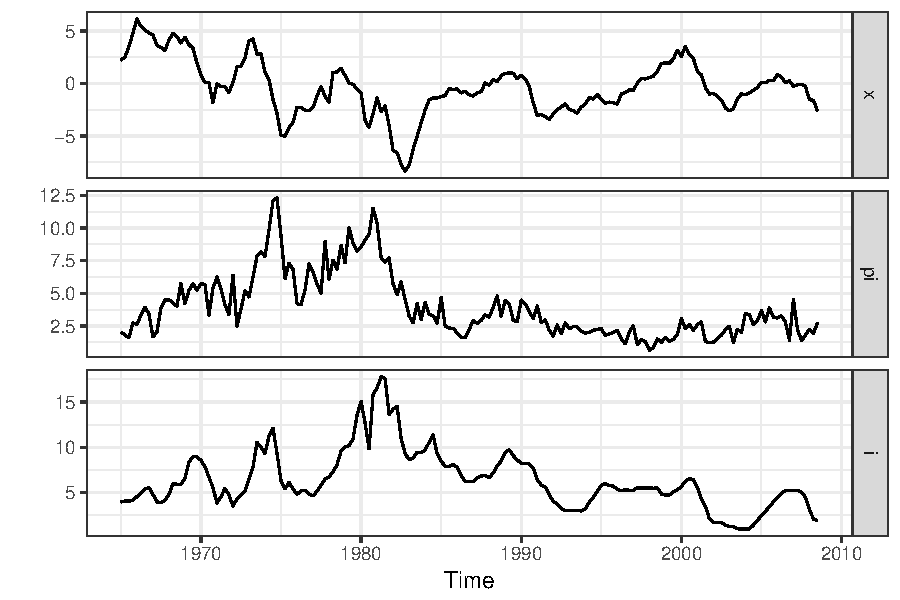
\includegraphics[scale=1]{Figures/USA_data}
\caption{US macroeconomic data.}
\label{fig:USA}
\end{figure}

The next step of the analysis is the estimation of the reduced form VAR, for instance, by means of the function \code{VAR()} from the \pkg{vars} package. We specify a VAR model with intercept of order $p = 6$. After model estimation, we can use the resulting \code{varest} object to estimate the structural form with the function \code{id.cv()}. We provide the structural break point with the function argument \code{SB} in \code{ts} date format.
\begin{CodeChunk}
\begin{CodeInput}
R> plain.var <- vars::VAR(USA, p = 6, type = 'const')
R> usa.cv <- id.cv(plain.var, SB = c(1979, 3))
R> summary(usa.cv)
\end{CodeInput}
\begin{CodeOutput}
Identification Results
----------------------

Method: Changes in Volatility
Sample size: 169
Likelihood: -564.2994
Structural Break: At Observation Number 59 during 1979 Q3
Number of GLS estimations: 21
Number of Restrictions: 0

Estimated unconditional Heteroscedasticity Matrix (Lambda):
        [,1]     [,2]     [,3]
x  0.3925906 0.000000 0.000000
pi 0.0000000 0.191641 0.000000
i  0.0000000 0.000000 1.244348

Standard Errors of Lambda:
         [,1]       [,2]      [,3]
x  0.09265819 0.00000000 0.0000000
pi 0.00000000 0.04527264 0.0000000
i  0.00000000 0.00000000 0.2935572

Estimated B Matrix (unique decomposition of the covariance matrix):
          [,1]       [,2]      [,3]
x   0.61193300 -0.5931964 0.2241237
pi  0.75559400  1.2987520 0.1131134
i  -0.02899916  0.1572953 0.7084709

Standard Errors of B:
        [,1]      [,2]       [,3]
x  0.1330924 0.1955350 0.07101215
pi 0.2498466 0.2600376 0.09960245
i  0.1559672 0.1213446 0.07004430

Pairwise Wald Test:
                  Test statistic p-value
lambda_1=lambda_2           3.80    0.05 *
lambda_1=lambda_3           7.66    0.01 **
lambda_2=lambda_3          12.56  <2e-16 ***
---
Signif. codes:  0 '***' 0.001 '**' 0.01 '*' 0.05 '.' 0.1 ' ' 1
\end{CodeOutput}
\end{CodeChunk}
The summary of the identified object displays the estimated decomposition of the covariance matrix $\widehat{B}$, as well as the covariance shift matrix $\widehat{\Lambda}$ and their corresponding standard errors. Moreover, the summary provides the results of pairwise Wald-type tests for distinct diagonal elements of $\widehat{\Lambda}$ which is necessary for unique identification of the structural shocks. In the present case, all three tests statistics yield a rejection of the null hypotheses of equal diagonal elements with 10\% significance. The ordering of the columns of $\widehat{B}$ is arbitrary and the user has to arrange them in an economically meaningful way. For instance,  \cite{HerwartzPloedt2016} order the columns according to a unique sign pattern which indicates the direction of the shocks on impact. The code below orders the columns in the same way.
\begin{CodeChunk}
\begin{CodeInput}
R> usa.cv$B <- usa.cv$B[, c(3, 2, 1)]
R> usa.cv$B[,3] <- usa.cv$B[, 3] * (-1)

R> usa.cv$B_SE <- usa.cv$B_SE[, c(3, 2, 1)]

R> usa.cv$Lambda <- diag(diag(usa.cv$Lambda)[c(3, 2, 1)])
R> usa.cv$Lambda_SE <- diag(diag(usa.cv$Lambda_SE)[c(3, 2, 1)])

R> round(usa.cv$B, 3)
\end{CodeInput}
\begin{CodeOutput}
    [,1]   [,2]   [,3]
x  0.224 -0.593 -0.612
pi 0.113  1.299 -0.756
i  0.708  0.157  0.029
\end{CodeOutput}
\begin{CodeInput}
R> round(usa.cv$Lambda, 3)
\end{CodeInput}
\begin{CodeOutput}
    [,1]  [,2]  [,3]
x  1.244 0.000 0.000
pi 0.000 0.192 0.000
i  0.000 0.000 0.393
\end{CodeOutput}
\end{CodeChunk}
\cite{HerwartzPloedt2016} interpret the impact effects in the first column of the matrix $\widehat{B}$ to characterize a demand shock. Similarly, the effects in the second (third) column indicate a supply (monetary policy) shock. The authors argue that their shock labeling according to the estmated sign patterns is in line with the relevant literature. Since the matrix $\widehat{\Lambda}$ represents the variance of structural shocks in the second regime, \cite{HerwartzPloedt2016} interpret the diagonal elements of $\widehat{\Lambda}$ such that the supply and monetary policy shocks have relatively lower variances and the demand shock a higher variance in regime two (i.e., for time instances $t>T_{SB} = 59$ or after the second quarter of 1979). The authors compare the results from this statistical identification scheme with a model structure implied by covariance decomposition matrix $B$ which is lower triangular by assumption \citep{Sims1980}. The \code{id.cv()} function enables the user to test for such restrictions by setting up a restriction matrix as described in the code below.
\begin{CodeChunk}
\begin{CodeInput}
restMat <- matrix(rep(NA, 9), ncol = 3)
restMat[1, c(2, 3)] <- 0
restMat[2, 3] <- 0
restMat
\end{CodeInput}
\begin{CodeOutput}
     [,1] [,2] [,3]
[1,]   NA    0    0
[2,]   NA   NA    0
[3,]   NA   NA   NA
\end{CodeOutput}
\begin{CodeInput}
R> restricted.model <- id.cv(plain.var, SB = c(1979, 3),
+    restriction_matrix = restMat)
R> summary(restricted.model)
\end{CodeInput}
\begin{CodeOutput}
Identification Results
----------------------

Method: Changes in Volatility
Sample size: 169
Likelihood: -568.6664
Structural Break: At Observation Number 59 during 1979 Q3
Number of GLS estimations: 23
Number of Restrictions: 3

Estimated unconditional Heteroscedasticity Matrix (Lambda):
        [,1]      [,2]      [,3]
x  0.3501948 0.0000000 0.0000000
pi 0.0000000 0.2346854 0.0000000
i  0.0000000 0.0000000 0.9420116

Standard Errors of Lambda:
         [,1]       [,2]     [,3]
x  0.08266738 0.00000000 0.000000
pi 0.00000000 0.05616318 0.000000
i  0.00000000 0.00000000 0.227189

Estimated B Matrix (unique decomposition of the covariance matrix):
         [,1]      [,2]      [,3]
x  0.87988465 0.0000000 0.0000000
pi 0.08137972 1.5306503 0.0000000
i  0.31518384 0.2606745 0.7378484

Standard Errors of B:
         [,1]       [,2]       [,3]
x  0.08638851 0.00000000 0.00000000
pi 0.10334026 0.15169565 0.00000000
i  0.08527442 0.08620187 0.07354585

Pairwise Wald Test:
                  Test statistic p-value
lambda_1=lambda_2           1.34    0.25
lambda_1=lambda_3           5.99    0.01 **
lambda_2=lambda_3           9.13  <2e-16 ***
---
Signif. codes:  0 '***' 0.001 '**' 0.01 '*' 0.05 '.' 0.1 ' ' 1

Likelihood Ratio Test:
 Test statistic p-value
          8.734   0.033 *
---
Signif. codes:  0 '***' 0.001 '**' 0.01 '*' 0.05 '.' 0.1 ' ' 1
\end{CodeOutput}
\end{CodeChunk}
Since the structural shocks are just identified by the change in the covariance matrix, any further restriction on $B$ over identifies the model and makes the restrictions testable. The function automatically performs a likelihood ratio test in case of such over identifying restrictions. The summary depicts the estimation results from the restricted model as well as the test statistics and $p$-values. The likelihood ratio test indicates that the null hypothesis of a lower triangular  structural impact matrix has to be rejected at the $5\%$ significance level. \cite{HerwartzPloedt2016} argue that identification by means of zero restrictions according to a lower triangular matrix lacks economic intuition which we can support with the obtained diagnostic. Therefore, the unrestricted model should be preferred for further analysis.

The next step is the calculation of impulse-response functions with boostrap confidence bands to investigate future effects of the
economically labeled structural shocks on the variables included in the model. Moreover, the implemented bootstrap functions allow for an evaluation of the significance of unique sign patterns in $\widehat{B}$ as described in \cite{HerwartzLDI2018}. We define a list of sign restrictions and label them as demand, supply and monetary policy shock respectively.
\begin{CodeChunk}
\begin{CodeInput}
R> signrest <- list(demand = c(1, 1, 1), supply = c(-1, 1, 1),
+    monetary_policy = c(-1, -1, 1))
\end{CodeInput}
\end{CodeChunk}
For illustration, we use the wild bootstrap implemented with a Rademacher distribution, fixed-design and $1000$ bootstrap replications as in \cite{HerwartzPloedt2016}. To reduce computation time we parallelize the bootstrap and specify a seed to obtain reproducible results. The time horizon for the impulse-response analysis has to be determined in advance using the argument \code{n.ahead}.
\begin{CodeChunk}
\begin{CodeInput}
R> cores <- parallel::detectCores() - 1
R> set.seed(231)
R> usa.cv.boot <- wild.boot(usa.cv, design = "fixed",
+  distr = "rademacher", nboot = 1000, n.ahead = 15,
+  nc = cores, signrest = signrest)
R> summary(usa.cv.boot)
\end{CodeInput}
\begin{CodeOutput}
Bootstrap Results
-----------------

Method: Wild bootstrap
Bootstrap iterations: 1000
Distribution used: rademacher
Design: fixed

Point estimates:
        [,1]       [,2]        [,3]
x  0.2241237 -0.5931964 -0.61193300
pi 0.1131134  1.2987520 -0.75559400
i  0.7084709  0.1572953  0.02899916

Bootstrap means:
         [,1]        [,2]       [,3]
x  0.08562671 -0.51047857 -0.6270604
pi 0.08586727  1.13181279 -0.7800737
i  0.69257452  0.02945994 -0.1839417

Bootstrap standard errors:
         [,1]      [,2]      [,3]
x  0.14112596 0.3093977 0.2501647
pi 0.16608174 0.4580203 0.5958669
i  0.07464771 0.2309445 0.2205195

Identified sign patterns:
=========================
Specified sign pattern:

   demand supply monetary_policy
x       1     -1              -1
pi      1      1              -1
i       1      1               1

Unique occurrence of single shocks according to sign pattern:
demand : 64.9 %
supply : 65 %
monetary_policy : 28.4 %

Joint occurrence of specified shocks: 12.7 %
\end{CodeOutput}
\begin{CodeInput}
R> plot(usa.cv.boot, lowerq = 0.16, upperq = 0.84)
\end{CodeInput}
\end{CodeChunk}
The summary reveals that only $12.7\%$ of all bootstrap estimates are in line with all economically motivated sign patterns jointly. The sign pattern of the monetary policy shock appears in only $28.4\%$ of all bootstrap samples. Furthermore, the bootstrap means indicate that the third shock is more in line with the sign pattern of the demand shock. This result is plausible noting that the point estimate in the lower right corner is close to zero and, therefore, lacks a significantly positive effect on the interest rate. Figure \ref{fig:irf_cv} shows the impulse-response functions of normalized shocks having unit variance in the first regime.
\begin{figure}[h]
\center
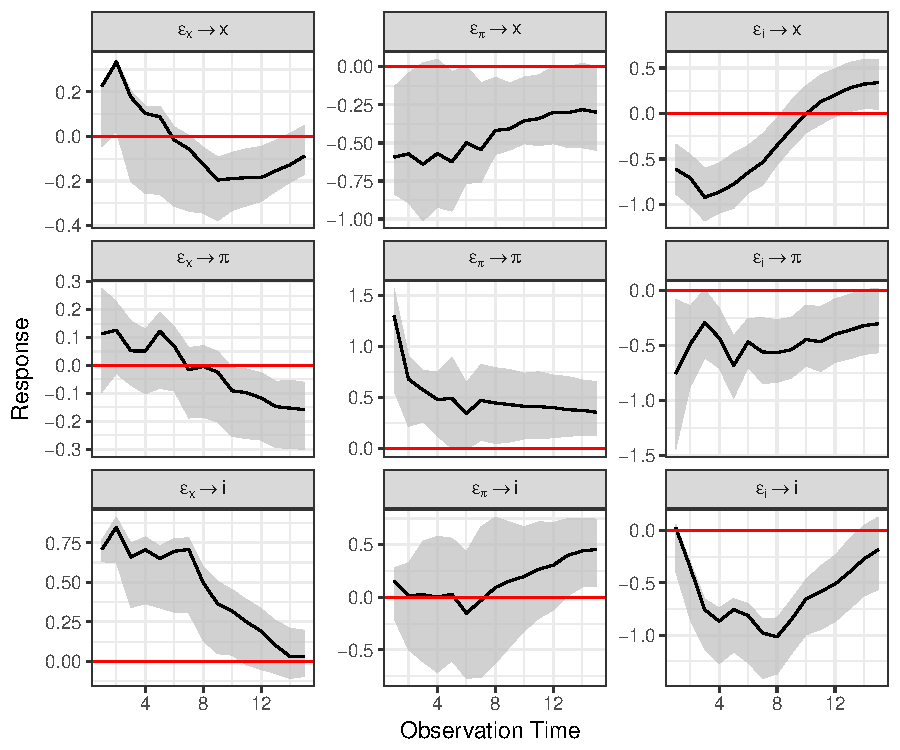
\includegraphics[scale=1]{Figures/IRF_cv}
\caption{Impulse-response functions with $68\%$ confidence bands based on $1000$ bootstrap replications. Structural shocks identified through unconditional shift in the covariance structure.}
\label{fig:irf_cv}
\end{figure}
\cite{HerwartzPloedt2016} argue that the negative reaction of the interest rate to a monetary policy shock after the initial period is implausible, and puts the interpretation of this shock as a monetary policy shock into question. The results from the bootstrap support the authors' argumentation with regard to the shock labeling. \\
Furthermore, we can calculate the forecast error variance decomposition to investigate the contribution of each shock to the prediction mean squared error of the variables. The \code{fevd()} method creates an object for visual inspection of the forecast error variance decomposition by means of the \code{plot} function.
\begin{CodeChunk}
\begin{CodeInput}
R> fev.cv <- fevd(usa.cv, n.ahead = 30)
R> plot(fev.cv)
\end{CodeInput}
\end{CodeChunk}
Figure \ref{fig:fev_cv} depicts the forecast error variance decomposition. It is evident that the monetary policy shock accounts for more than $50\%$ of the prediction mean squared error of the output gap, whereas the demand shock constantly accounts for only about $5\%$ of the prediction mean squared error. Moreover, the demand shock contributes almost $100\%$ of the forecast error variance of the interest rates on impact.
\begin{figure}[h]
\center
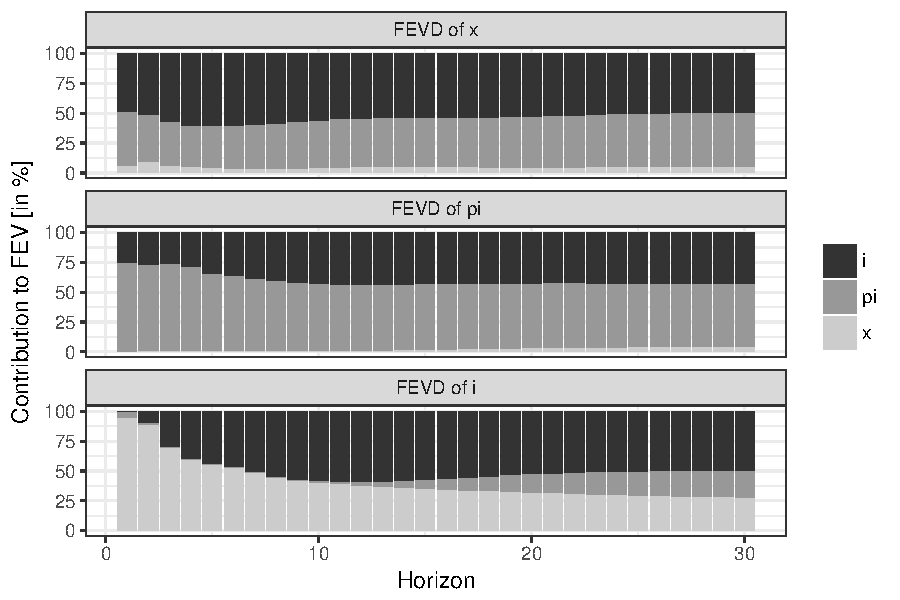
\includegraphics[scale=1]{Figures/FEV_cv}
\caption{Forecast error variance decomposition for $30$ periods. Structural shocks identified by means of the CV model.}
\label{fig:fev_cv}
\end{figure}
Thus, the forecast error decompositions hint at a shock labeling which differs from the one developed above on the basis of sign patterns of  $\widehat{B}$. Furthermore, they confirm the conclusion of \cite{HerwartzPloedt2016} that the empirical model fails to identify a monetary policy shock according to its theoretical effect patterns.\\

We re-estimate the structural form with the DC method under the assumption of independent non-Gaussian shocks.\footnote{Component-wise kurtosis and skewness tests as implemented in the package \pkg{normtest} \citep{normtest} as well as fourth-order blind identification based tests from the package \pkg{ICtest} \citep{ICtest} show no indication for Gaussian components.}
\begin{CodeChunk}
\begin{CodeInput}
R> usa.dc <- id.dc(plain.var, PIT = FALSE)
R> summary(usa.dc)
\end{CodeInput}
\begin{CodeOutput}
Identification Results
----------------------

Method: Distance covariances
Sample size: 169

Estimated B Matrix (unique decomposition of the covariance matrix):
          [,1]        [,2]      [,3]
x  0.541926899 -0.36707854 0.1964223
pi 0.508827712  0.92428628 0.1967426
i  0.003560267  0.02576151 0.8194037
\end{CodeOutput}
\end{CodeChunk}
The estimated structural matrix differs from the estimated matrix obtained from the CV approach. The matrix identified by means of the DC method does not allow for a labelling of the shocks that accords with a unique sign pattern. Nevertheless, it is possible to label the shocks in a meaningful way, since one could assume that the loading of the structural shocks on reduced form errors is stronger for own effects in comparison with cross variable effects. The finding that a positive monetary policy shock has a positive effect on output and inflation might seem to be at odds with intuition at first, although this mechanism can be observed rather frequently in the literature \citep[e.g.,][]{LUTKEPOHL20172} and is usually referred to as a so-called price puzzle \citep{E1992}. Conditional on the estimate $\widehat{B}$, we construct the historical decomposition. As an example, we decompose the output into its underlying determinants over the sample period. In the data set output is the first column and, hence, \code{series = 1} is the provided option.
\begin{CodeChunk}
\begin{CodeInput}
R> hd.cv.1 <- hd(usa.dc, series = 1)
R> plot(hd.cv.1)
\end{CodeInput}
\end{CodeChunk}
Figure \ref{fig:hd_dc} indicates that output fluctuations are mainly explained by demand shocks rather than supply or monetary policy shocks.
\begin{figure}[h]
\center
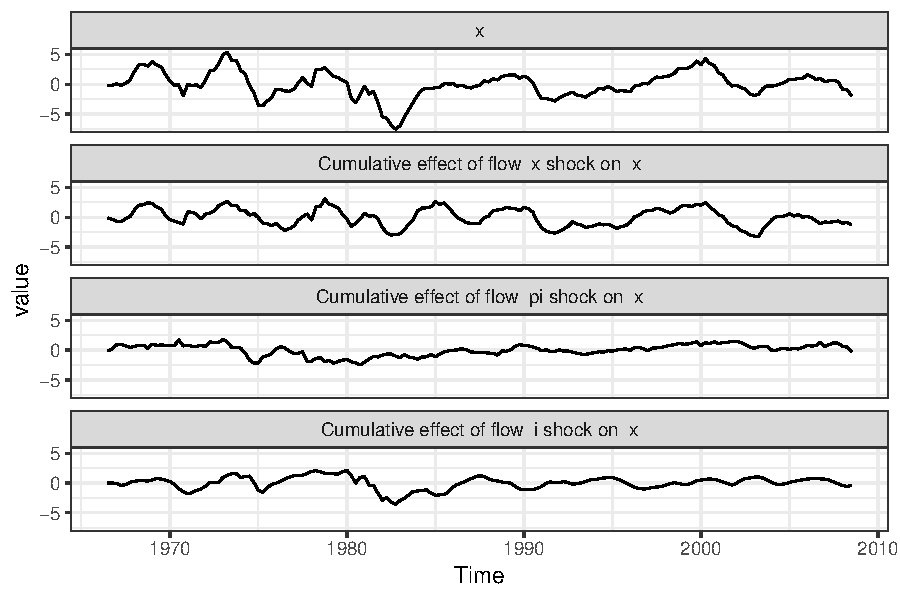
\includegraphics[scale=1]{Figures/hd_dc}
\caption{Historical decomposition of the US output gap in percent deviations from the mean. Structural shocks are identified by means of the DC algorithm.}
\label{fig:hd_dc}
\end{figure}

%% -- Summary/conclusions/discussion -------------------------------------------
\section{Summary} \label{sec:summary}
The \proglang{R} package \pkg{svars} provides a vast set of estimation techniques that build on several assumptions on the data and a variety of input arguments. In the present article we describe how the implemented identification techniques for SVAR models depend on assumptions of heteroskedasticity and independence coupled with non-Gaussianity to retrieve the structural shocks from the reduced form VAR model. Furthermore, we provide a set of auxiliary functions which complement the cornerstone identification methods, and thereby  offer a complete toolbox for structural analysis in a multivariate time series context.\\

We give a step-by-step guideline on how to use the functions on a real dataset comparing one representative from both groups of heteroskedasticity and independence based identification.
Even though the estimation results are similar, identification by means of covariance shifts might imply a misleading sign pattern which is indicated in the forecast error variance decomposition. Moreover, we illustrate how to test sign and zero restrictions by means of restricted log-likelihood estimation and bootstrap methods.\\

The \pkg{svars} package contains six alternative and recent SVAR identification techniques. Besides these, further popular data-driven identification approaches include, e.g., the heteroskedastic model with Markov switching mechanisms \citep{LanneLuetMac2010, HerwartzLuetkepohl2014} or pseudo ML estimation \citep{PML}. Moreover, an option to test for long run restrictions by means of likelihood based identification schemes is a possible augmentation of the package. We regard both directions as promising for future developments of \pkg{svars}.

%% -- Optional special unnumbered sections -------------------------------------

%\section*{Computational details}
%
%The results in this paper were obtained using
%\proglang{R}~3.4.1 with the
%\pkg{MASS}~7.3.47 package. \proglang{R} itself
%and all packages used are available from the Comprehensive
%\proglang{R} Archive Network (CRAN) at
%\url{https://CRAN.R-project.org/}.


\section*{Acknowledgments}

We thank the editors and two anonymous reviewers for helpful comments and suggestions. Furthermore, we thank Bernhard Pfaff for his kind help. Financial support of the DFG through project HE 2188/12-1 and 192626868 as well as the Academy of Finland (308628) are gratefully acknowledged.


%
%\begin{leftbar}
%All acknowledgments (note the AE spelling) should be collected in this
%unnumbered section before the references. It may contain the usual information
%about funding and feedback from colleagues/reviewers/etc. Furthermore,
%information such as relative contributions of the authors may be added here
%(if any).
%\end{leftbar}


%% -- Bibliography -------------------------------------------------------------
%% - References need to be provided in a .bib BibTeX database.
%% - All references should be made with \cite, \citet, \citep, \citealp etc.
%%   (and never hard-coded). See the FAQ for details.
%% - JSS-specific markup (\proglang, \pkg, \code) should be used in the .bib.
%% - Titles in the .bib should be in title case.
%% - DOIs should be included where available.

\bibliography{refs}


%% -- Appendix (if any) --------------------------------------------------------
%% - After the bibliography with page break.
%% - With proper section titles and _not_ just "Appendix".



%% -----------------------------------------------------------------------------


\end{document}
